% !TEX program = xelatex
%----------------------- Преамбула -----------------------
\documentclass[utf8x, 14pt, oneside, a4paper]{article}

\usepackage{extsizes} % Для добавления в параметры класса документа 14pt

% Для работы с несколькими языками и шрифтом Times New Roman по-умолчанию
\usepackage[english,russian]{babel}
%\usepackage{fontspec}
%\setmainfont{Times New Roman}
\usepackage{pscyr}
\renewcommand{\rmdefault}{ftm}
% ГОСТовские настройки для полей и абзацев
\usepackage[left=30mm,right=15mm,top=20mm,bottom=20mm]{geometry}
\usepackage{misccorr}
\usepackage{indentfirst}
\usepackage{enumitem}
\setlength{\parindent}{1.25cm}
\linespread{1.3}
\setlist{nolistsep} % Отсутствие отступов между элементами \enumerate и \itemize

% Дополнительное окружения для подписей
\usepackage{array}
\newenvironment{signstabular}[1][1]{
	\renewcommand*{\arraystretch}{#1}
	\tabular
}{
	\endtabular
}

% Переопределение стандартных \section, \subsection, \subsubsection по ГОСТу;
% Переопределение их отступов до и после для 1.5 интервала во всем документе
\usepackage{titlesec}

\titleformat{\section}[block]
{\bfseries\normalsize\filcenter}{\thesection}{1em}{}

\titleformat{\subsection}[hang]
{\bfseries\normalsize}{\thesubsection}{1em}{}
\titlespacing\subsection{\parindent}{\parskip}{\parskip}

\titleformat{\subsubsection}[hang]
{\bfseries\normalsize}{\thesubsubsection}{1em}{}
\titlespacing\subsubsection{\parindent}{\parskip}{\parskip}

% Работа с изображениями и таблицами; переопределение названий по ГОСТу
\usepackage{caption}
\captionsetup[figure]{name={Рисунок},labelsep=endash}
\captionsetup[table]{singlelinecheck=false, labelsep=endash}

\usepackage{graphicx}
%\usepackage{slashbox} % Диагональное разделение первой ячейки в таблицах

% Цвета для гиперссылок и листингов
\usepackage{color}

% Гиперссылки \toc с кликабельностью
\usepackage{hyperref}

\hypersetup{
	linktoc=all,
	linkcolor=black,
	urlcolor=black,
	citecolor=black,
	colorlinks=true,
}

% Листинги
%\setsansfont{Arial}
%\setmonofont{Courier New}

\usepackage{color} % Цвета для гиперссылок и листингов
\definecolor{comment}{rgb}{0,0.5,0}
\definecolor{plain}{rgb}{0.2,0.2,0.2}
\definecolor{string}{rgb}{0.91,0.45,0.32}

\usepackage{listings}
\lstset{
	basicstyle=\footnotesize\ttfamily,
	language=[Sharp]C, % Или другой ваш язык -- см. документацию пакета
	commentstyle=\color{comment},
	numbers=left,
	numberstyle=\tiny\color{plain},
	numbersep=5pt,
	tabsize=4,
	extendedchars=\true,
	breaklines=true,
	keywordstyle=\color{blue},
	frame=b,
	stringstyle=\ttfamily\color{string}\ttfamily,
	showspaces=false,
	showtabs=false,
	xleftmargin=17pt,
	framexleftmargin=17pt,
	framexrightmargin=5pt,
	framexbottommargin=4pt,
	showstringspaces=false,
	inputencoding=utf8x,
	keepspaces=true
}

\DeclareCaptionLabelSeparator{line}{\ --\ }
\DeclareCaptionFont{white}{\color{white}}
\DeclareCaptionFormat{listing}{\colorbox[cmyk]{0.43,0.35,0.35,0.01}{\parbox{\textwidth}{\hspace{15pt}#1#2#3}}}
\captionsetup[lstlisting]{
	format=listing,
	labelfont=white,
	textfont=white,
	singlelinecheck=false,
	margin=0pt,
	font={bf,footnotesize},
	labelsep=line
}
%%% Дополнительная работа с математикой
\usepackage{amsfonts,amssymb,amsthm,mathtools} % AMS
\usepackage{amsmath}
\usepackage{icomma} % "Умная" запятая: $0,2$ --- число, $0, 2$ --- перечисление

%% Номера формул
%\mathtoolsset{showonlyrefs=true} % Показывать номера только у тех формул, на которые есть \eqref{} в тексте.

%% Шрифты
\usepackage{euscript}	 % Шрифт Евклид
\usepackage{mathrsfs} % Красивый матшрифт

%% Свои команды
\DeclareMathOperator{\sgn}{\mathop{sgn}}

%% Перенос знаков в формулах (по Львовскому)
\newcommand*{\hm}[1]{#1\nobreak\discretionary{}
{\hbox{$\mathsurround=0pt #1$}}{}}

%%% Работа с картинками
\usepackage{float}
\usepackage{graphicx}  % Для вставки рисунков
\graphicspath{{pictures/}}  % папки с картинками
\setlength\fboxsep{3pt} % Отступ рамки \fbox{} от рисунка
\setlength\fboxrule{1pt} % Толщина линий рамки \fbox{}
\usepackage{wrapfig} % Обтекание рисунков и таблиц текстом

%%% Работа с таблицами
\usepackage{array,tabularx,tabulary,booktabs} % Дополнительная работа с таблицами
\usepackage{longtable}  % Длинные таблицы
\usepackage{multirow} % Слияние строк в таблице

\usepackage{cite}
\usepackage{csquotes}
% Годные пакеты для обычных действий
\usepackage{ulem} % Нормальное нижнее подчеркивание
\usepackage{hhline} % Двойная горизонтальная линия в таблицах
\usepackage[figure,table]{totalcount} % Подсчет изображений, таблиц
\usepackage{rotating} % Поворот изображения вместе с названием
\usepackage{lastpage} % Для подсчета числа страниц
\usepackage{ragged2e}
\justifying





\usepackage[square,numbers,sort&compress]{natbib}
\renewcommand{\bibnumfmt}[1]{#1.\hfill} % нумерация источников в самом списке — через точку
\renewcommand{\bibsection}{\section*{СПИСОК ИСПОЛЬЗОВАННЫХ ИСТОЧНИКОВ}} % заголовок специального раздела
\setlength{\bibsep}{0pt}










% ---------------------- Документ ----------------------
\begin{document}
	\begin{titlepage}
		\noindent\begin{minipage}{0.05\textwidth}
			
\includegraphics[scale=0.3]{1.png}
		\end{minipage}
		\hfill
		\begin{minipage}{0.85\textwidth}\raggedleft
			\begin{center}
				\fontsize{12pt}{0.3\baselineskip}\selectfont \textbf{Министерство науки и высшего образования Российской Федерации \\ Федеральное государственное бюджетное образовательное учреждение \\ высшего образования \\ <<Московский государственный технический университет \\ имени Н.Э. Баумана \\ (национальный исследовательский университет)>> \\ (МГТУ им. Н.Э. Баумана)}
			\end{center}
		\end{minipage}

		\begin{center}
			\fontsize{12pt}{0.1\baselineskip}\selectfont
			\noindent\makebox[\linewidth]{\rule{\textwidth}{4pt}} \makebox[\linewidth]{\rule{\textwidth}{1pt}}
		\end{center}

		\begin{flushleft}
			\fontsize{12pt}{0.8\baselineskip}\selectfont 
			
			ФАКУЛЬТЕТ \uline{<<\textbf{<Факультет (полностью)>}>> \hfill}

			КАФЕДРА \uline{\hspace{4mm} <<\textbf{<Кафедра (полностью)>}>> \hfill}
		\end{flushleft}

		\vfill

		\begin{center}
			\fontsize{20pt}{\baselineskip}\selectfont

			\textbf{РАСЧЕТНО-ПОЯСНИТЕЛЬНАЯ ЗАПИСКА}

			\textbf{\textit{К ВЫПУСКНОЙ КВАЛИФИКАЦИОННОЙ РАБОТЕ}}

			\textbf{\textit{НА ТЕМУ:}}
		\end{center}

		\begin{center}
			\fontsize{18pt}{0.6cm}\selectfont 
			
			\uline{\hfill}
	
			\uline{\hfill}
	
			\uline{\hfill}
	
			\uline{\hfill}
	
			\uline{\hfill}
		\end{center}

		\vfill

		\begin{table}[h!]
			\fontsize{12pt}{0.7\baselineskip}\selectfont
			\centering
			\begin{signstabular}[0.7]{p{7.25cm} >{\centering\arraybackslash}p{4cm} >{\centering\arraybackslash}p{4cm}}
				Студент группы \textbf{<Группа (Шифр)>} & \uline{\hspace*{4cm}} & \uline{\hfill \textbf{<И.О. Фамилия>} \hfill} \\
				& \scriptsize (Подпись, дата) & \scriptsize (И.О. Фамилия)
			\end{signstabular}

			\vspace{\baselineskip}

			\begin{signstabular}[0.7]{p{7.25cm} >{\centering\arraybackslash}p{4cm} >{\centering\arraybackslash}p{4cm}}
				Руководитель ВКР & \uline{\hspace*{4cm}} & \uline{\hfill \textbf{<И.О. Фамилия>} \hfill} \\
				& \scriptsize (Подпись, дата) & \scriptsize (И.О. Фамилия)
			\end{signstabular}

			\vspace{\baselineskip}

			\begin{signstabular}[0.7]{p{7.25cm} >{\centering\arraybackslash}p{4cm} >{\centering\arraybackslash}p{4cm}}
				Нормоконтроллер & \uline{\hspace*{4cm}} & \uline{\hfill \textbf{<И.О. Фамилия>} \hfill} \\
				& \scriptsize (Подпись, дата) & \scriptsize (И.О. Фамилия)
			\end{signstabular}
		\end{table}

		\vfill

		\begin{center}
			\normalsize \textit{\textbf{<Год>} г.}
		\end{center}
	\end{titlepage}
\pagebreak
	\normalsize
	\setcounter{page}{2}
	
		\section*{РЕФЕРАТ}
		\addcontentsline{toc}{section}{РЕФЕРАТ}
		\normalsize
			Расчетно-пояснительная записка \pageref{LastPage} с., \totalfigures\ рис., \totaltables\ табл., 15 ист., 1 прил.

			\textbf{<Ключевые слова>}
			
ПРОКАЛОЧНЫЕ ПЕЧИ, ЮВЕЛИРНЫЕ УКРАШЕНИЯ, ЛИТЬЕ ПО ВЫПЛАВЛЯЕМЫМ МОДЕЛЯМ, ФУТЕРОВКА.

Объектом разработки является прокалочная печь для ювелирного литья.

Цель работы -- модернизация прокалочной печи для уменьшения расхода энергии, затрачиваемой на нагрев печи.

Поставленная цель достигается за счет применения улучшенной футеровки печи и дверцы загрузочного окна, улучшения герметизации рабочего пространства печи за счет наклонной дверцы, замены нихромовых нагревательных элементов на силитовые стержни с целью создания стабильного температурного поля по сечению печи.


		\pagebreak
	
	% Переопределяем название \toc и выводим сам \toc
	\renewcommand{\contentsname}{\normalsize\bfseries\centering СОДЕРЖАНИЕ}
	\small
	\tableofcontents
	\normalsize

		\pagebreak

	\section*{ВВЕДЕНИЕ}
		\addcontentsline{toc}{section}{ВВЕДЕНИЕ}


\subsection*{Введение в метод дискретных элементов}

Впервые метод дискретных элементов (в дальнейшем МДЭ или DEM) был предложен в 1971 году инженерами Cundall P. A. и Otto D. L. Strack \cite{cundall} для моделирования поведения мелких частиц горных пород. 
МДЭ представляет собой совокупность методов для изучения сыпучих сред. 

Сыпучими средами вполне можно назвать любые дискретизированные среды (песок, грунт, зерно и пр.). 
Сыпучая среда сложна в аналитическом представлении, потому что в зависимости от многих факторов она может проявлять твердоподобное, жидкоподобное или комбинированное свойства. 

\begin{figure}[H]
	\centering
	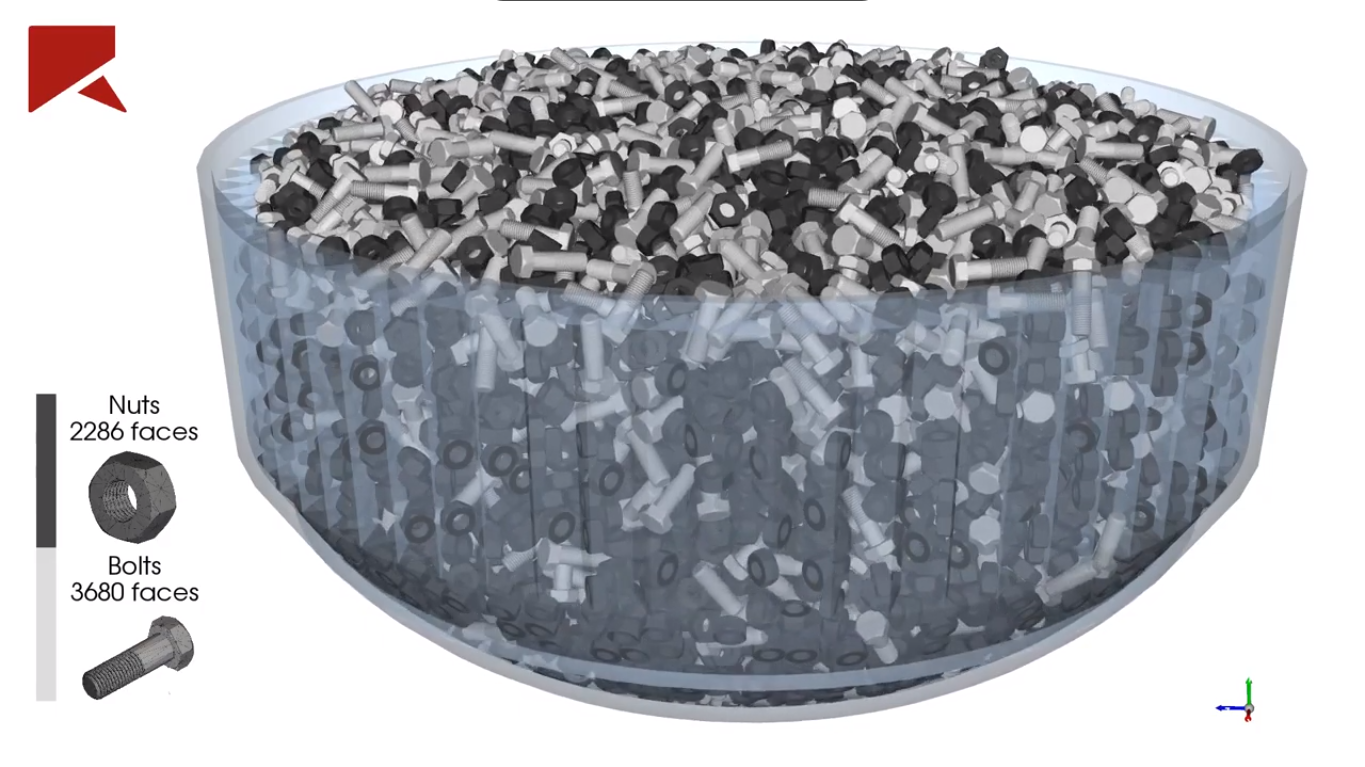
\includegraphics[width=0.5\textwidth]{sreda}
	\caption{Демонстрация сыпучей среды (в данном случае болты и гайки тоже являются сыпучей средой).}
\end{figure} 

Численный расчёт для сыпучих сред проводится независимо для каждого элемента, а взаимодействуют они [элементы] только в точках контакта. 
Основываясь на всем вышесказанном в 1971 году и появился метод дискретных элементов.

Уже на данном этапе мы можем выделить основные преимущество и недостаток данного метода. 
Преимуществом можно назвать возможность моделирования ситуации и сыпучей среды любой сложности без проведения сложных дорогостоящих экспериментов. 
Недостатком же является высокая требовательность к вычислительным ресурсам.

В общем виде работа алгоритма представлена на рисунке \ref{pic:algo}.

Метод дискретных элементов может рассматриваться как обобщение метода конечных элементов \cite{mde_smth}.
Он был разработан и впервые применен для исследования механики горных пород. 
При моделировании процесса этим методом задаются начальные положения и скорости частиц. 
Затем, исходя из этих начальных данных и также задаваемых физических законов взаимодействия частиц, вычисляются силы, действующие на каждую частицу. 
При этом можно учитывать самые различные законы взаимодействия; достаточно, чтобы для их описания существовали разрешимые уравнения. 
Для каждой частицы вычисляется результирующая сила и также решается задача Коши на выбранном отрезке времени. 
В результате получаются начальные данные для следующего шага.
Вычисления продолжаются в течение всего представляющего интерес времени протекания процесса. 
Провести четкую границу между методом динамики частиц и методом дискретных элементов сложно; основное различие состоит в том, что первый возник как обобщение метода молекулярной динамики, а второй – как обобщение метода конечных элементов. 
Однако в настоящее время оба метода могут приводить фактически к одинаковым вычислительным алгоритмам, и название в основном определяется тем, какие пакеты программ используются для расчета.

\begin{figure}[H]
	\centering
	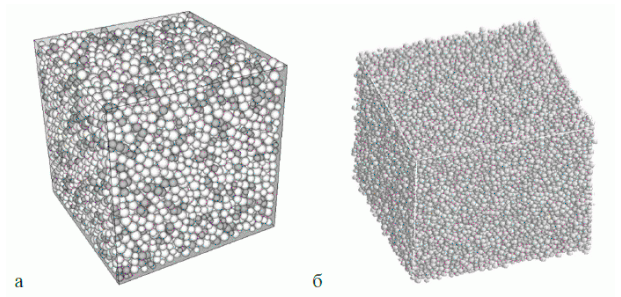
\includegraphics[width=0.8\textwidth]{primer}
	\caption{Модель плотной упаковки сфер по методу дискретных элементов: 10000 частиц (а); 30000 частиц (б)}
\end{figure} 

Безусловно, при вычислении движений каждой частицы описанными методами возникают необратимые погрешности, а задача вычисления индивидуальных траекторий принципиально нелинейна и неустойчива.
Однако, исходя из физических соображений, можно ожидать, что эти обстоятельства не повлияют на макроскопическую усредненную картину процесса. 

Основные перспективы использования методов при исследовании и оптимизации процессов переработки природных и техногенных материалов это:

--- вибрационное транспортирование сыпучих материалов;

--- вибрационная сегрегация и грохочение сыпучих материалов;

--- измельчение в барабанных мельницах;

--- дробление в щековых и конусных дробилках и др.

\begin{figure}[H]
	\centering
	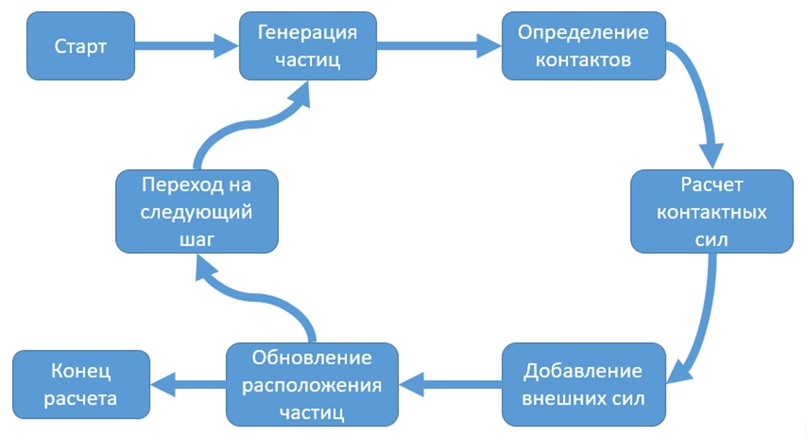
\includegraphics[width=0.7\textwidth]{algorithm}
	\caption{Алгоритм метода в общем виде}
	\label{pic:algo}
\end{figure} 

\subsection*{Обзор поставленных задач}

Существует два подхода к моделированию взаимодействия частиц: расчет скоростей на основе использования закона сохранения импульса, а также прямое рассмотрение контактного взаимодействия. В первом подходе принимается, что контактное взаимодействие происходит мгновенно, учет диссипации энергии производится за счет введения специальных эмпирических коэффициентов (коэффициентов восстановления) в закон сохранения импульса, уменьшающих скорости частиц после соударения \cite{cundall}.

На каждом шаге по времени для найденных взаимодействий происходит расчёт соответствующих контактных сил.
Существует несколько различных моделей силы контакта, подходящих для различных применений, материалов и условий \cite{hard_aglomerath}.

\begin{figure}[H]
	\centering
	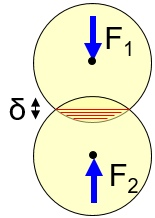
\includegraphics[width=0.3\textwidth]{vhod}
	\caption{Демонстрация контактных сил при пересечении двух шаров.}
\end{figure} 

Силы, действующие на каждую частицу, вычисляются из исходных данных, соответствующих физических законов и выбранной модели контакта (модели контакта необходимо выбирать исходя из условий применения) \cite{some}. 
В случае необходимости к расчёту могут быть подключены дополнительные модели: модель когезии, модель демпфирования и т.п., так же хотелось бы отметить что в расчёте могут иметь влияние такие силы, как:

--- трение, при касании двух частиц;

--- отскакивание, при столкновении;

--- гравитация;

--- притяжение (адгезия, жидкостное соединение).

После определения контактных сил, могут быть добавлены любые другие силы внешнего тела. 
Внешние силы возникают из-за существования одного или нескольких физических полей, таких как гравитационные, электромагнитные или гидродинамические поля.

После нахождения результирующей силы, взаимодействующей на каждую частицу, основываясь на втором законе Ньютона, находится новая позиция всех частиц к началу следующего шага по времени.
Временной шаг сменяется на следующий и цикл повторяется.

В данной работе помимо расчёта контактных сил действующих друг на друга также вводятся гравитационное поле, учёт сил трения, а также модель демпфирования. 
В качестве рассматриваемой модели принимается сферическое тело.

Частицы в данной работе будут представлять собой набор руды и дроби, перемещающийся в барабанной мельнице.
Т.к. задача решается для трех степеней свободы (две линейных и одна угловая), то это будет выглядеть как проекция посередине барабанной мельницы. Именно посередине -- во избежания различных краевых эффектов. Сама мельница будет представлена в виде набора прямых линий, составляющих замкнутую фигуру (в данном конкретном случае -- правильный многоугольник). Если уменьшать размер линий, то фигура будет стремиться к кругу, но принципиально это не повлияет на режим работы мельницы, а кратно увеличить время работы программы способно, поэтому дробление происходит до разумных пределов.

При моделировании барабанной мельницы также необходимо обеспечить появление новых частиц руды и исчезновение достаточно малых частиц, попавших в зону сита.
В двухмерной постановке задачи приходится прибегать к определенным хитростям, чтобы отобразить перемещения по третьей оси.
Подавать частицы мы будем равномерно.
С четко заданной переодичностью в местах предположительно меньшего количества шаров будут появляться частицы руды.
В свою очередь в центре есть зона при попадании в которую маленькие частицы будут исчезать из дальнейшего расчета (проходить через сита и идти дальше на обработку).


\subsection*{Современное состояние метода дискретных элементов}

Метод дискретных элементов не ограничивает расчёт только сферическими телами. 
Для создания тел любой другой сложной формы можно представить множеством элементов сфер, жёстко связанных между собой (мультисферный агломерат) \cite{aglomerath}.
Современный расчет предполагает именно такой подход для моделирования трехмерных тел случайной формы и оболочек.
Можно так же представить какое-либо тело в виде множества частиц более сложной формы (многоугольников). 
Этот подход требует большую ресурсоемкость и используется в узких задачах где необходима большая точность и есть относительно четкое представление о форме полученных частиц.
На рисунке \ref{pic:aglomerath} справа налево представлено упрощение сложной частицы до семи сфер жестко связанных друг с другом.
\begin{figure}[H]
	\centering
	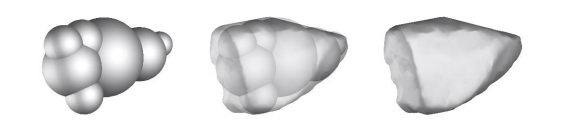
\includegraphics[width=0.8\textwidth]{aglomerath}
	\caption{Мультисферное изображение частицы сложной формы \cite{another_hard}}
	\label{pic:aglomerath}
\end{figure} 

В системах, где условия нагружения не оказывают существенного влияния на целостность частиц, не требуется специальной модели разрушения. 
В этих случаях обычно используются модели Герца или линейные пружинные контакты. 
Однако при использовании МДЭ для понимания механизмов в устройствах для измельчения, где целью является разрушение твердых частиц, необходим подход моделирования разрушения.
Задача моделирования частиц руды в барабанной мельнице является именно такой задачей.
Существует три основных подхода \cite{another_hard} к прерывному моделированию разрушения горных пород (остальные методы -- их вариации):

--- модель связанных частиц (BPM) - сферы собраны в кластер и соединены вместе в каждой точке контакта с помощью связывающих балок.
 
--- модель полиэдрических элементов (PEM) - частицы моделируются с использованием мозаичной структуры сетки с использованием зерен вороного, тригонов или тетраэдрических элементов.
 
--- модель замещения баланса популяции (PBRM) - частицы заменяются набором дочерних фрагментов в момент разрушения.
\begin{figure}[H]
	\centering
	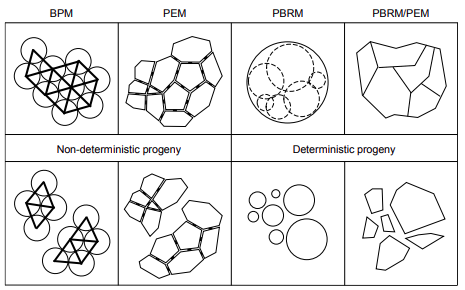
\includegraphics[width=0.6\textwidth]{break_model}
	\caption{Схематическое представление моделей разрушения \cite{another_hard}}
	\label{pic:break_model}
\end{figure} 
Все три из этих подходов, показанных на рисунке \ref{pic:break_model}, использовались для моделирования разрушения горных пород в измельчающих машинах. 
BPM применялся для моделирования разрушения горных пород, гранул и бетонных материалов с использованием режимов ударного разрушения и режимов разрушения при сжатии.
Некоторые инженеры \cite{another_hard} также смоделировали машины для измельчения, такие как, например, конусная дробилка, используя подход PBRM. 
Они использовали альтернативный подход к представлению сферической или многогранной формы. 
Применяется метод, при котором набор гладких угловых кубоидов с заранее определенным распределением размеров упаковывается внутри исходной кубоидной частицы.

В данной работе используется модель замещения баланса популяции (PBRM).

Большинство современного программного обеспечения для инженерных расчётов имеет в себе встроенные МДЭ решатели (Ansys Fluent, LS-DYNA), в свою очередь ПО специализирующееся на МДЭ (ESSS Rocky, open-source LIGGGHTS, EDEM (DEM Solutions Ltd.)), зачастую имеет большее широкий спектр возможностей для расчёта поведения сыпучей среды, таких как большее количество моделей контактных сил.

\begin{figure}[H]
	\centering
	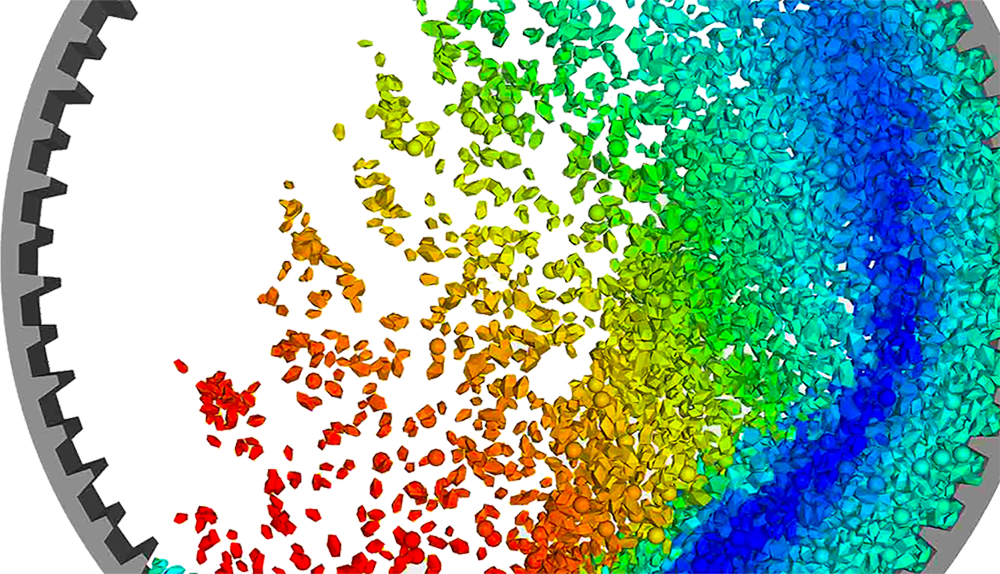
\includegraphics[width=0.8\textwidth]{rocky_dem_j}
	\caption{Пример моделирования частиц рудоразмольной мельницы в програмной среде Rocky DEM}
	\label{pic:rocky}
\end{figure} 


За счёт использования GPU (имеющих большее количество вычислительных ядер), большинство программ преодолело миллион частиц, которые одновременно могут находиться в области расчёта \cite{another_hard}. 
Распараллеливание процессов и введение многопоточной работы может заметно ускорить работу данного итерационного расчёта \cite{priklad}.

\subsection*{Барабанная мельница}
\label{mill_theory}

\begin{figure}[H]
	\centering
	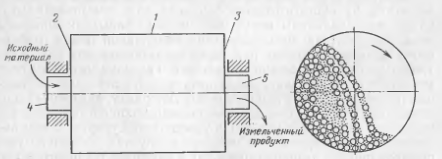
\includegraphics[width=0.8\textwidth]{baraban_shema}
	\caption{Схема барабанной мельницы}
	\label{pic:baraban_shema}
\end{figure} 

Барабанная мельница (рисунок \ref{pic:baraban_shema}) представляет собой пустотелый барабан 1, закрытый торцевыми крышками 2 и 3, в центре которых имеются полые цапфы 4 и 5. 
Цапфы опираются на подшипники и барабан вращается вокруг горизонтальной оси.
Барабан заполняется примерно на половину объема дробящей средой.
При его вращении дробящие тела  благодаря трению увлекаются его внутренней поверхностью, поднимаются на некоторую высоту и свободно или перекатываясь падают вниз \cite{china_mill}.
Материал измельчается в результате удара при относительно быстром перемещении мелющих тел и частиц материала.
Через одну полую цапфу внутрь барабана непрерывно подается измельчаемый материал, который проходит вдоль него и, подвергаясь воздействию дробящих тел, измельчается ударом, истиранием и раздавливанием.
Измельченный продукт непрерывно разгружается через другую полую цапфу \cite{mill_book}.

Применяется в основном в горнорудной промышленности, для создания порошка для использования в красках, пиротехнических средствах, пищевой промышленности и в керамике. 
Барабанные мельницы используются при производстве цемента, извести, гипса, керамических изделий, орехов, сахара и т. п. для измельчения материала до частиц размером менее десятых долей миллиметра. 
Процесс помола отличается большой энергоёмкостью и стоимостью \cite{mill_smth}. 
А режим работы шаровой мельницы характеризуется частотой вращения барабана. 
Для того чтобы экспериментально найти оптимальный режим работы может уйти довольно много ресурсов и времени.

		\pagebreak

\section{Основная часть. Построение математической модели}

\subsection{Упрощения метода дискретных элементов}
В алгоритме МДЭ, использованном в данной работе, есть несколько основных упрощений. 

1) Метод дискретных элементов основан на идее, что выбранный временной шаг настолько мал, что в течение одного временного шага \textbf{возмущения не могут распространяться с любого элемента дальше, чем на его ближайших соседей}. 
Тогда во все времена результирующие силы на любом элементе определяются исключительно его взаимодействием с элементами, с которыми он находится в контакте.
Именно эта ключевая особенность метода отдельных элементов позволяет проследить нелинейное взаимодействие большого числа дисков без чрезмерных требований к памяти.

\begin{figure}[H]
	\centering
	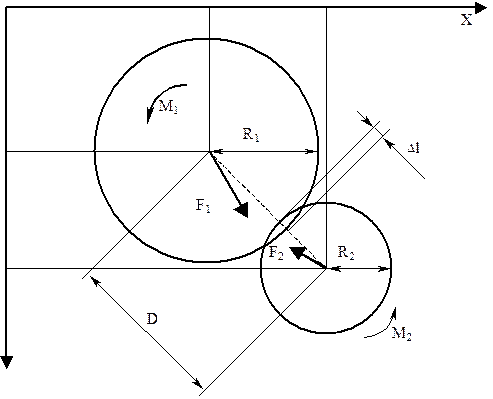
\includegraphics[width=0.8\textwidth]{entry_pic}
	\caption{Взаимодействие двух частиц в методе дискретных элементов.}
	\label{pic:entry_pic}
\end{figure} 


2) \textbf{Считается, что шары не деформируются.}
Деформации отдельных частиц малы по сравнению с изменением объёма дискретной среды в целом.
Поэтому точное моделирование деформации частиц не является необходимым для получения хорошей аппроксимации механического поведения. 
В данном методе частицам разрешено перекрывать друг друга в точках соприкосновения. 
Это перекрывающее поведение занимает место деформации отдельных частиц. 
Величина перекрытия напрямую связана с контактной силой, как будет описано ниже.
Однако следует отметить, что эти перекрытия малы по отношению к размерам частиц.
Таким образом, мы отказываемся от рассмотрения НДС внутри частиц в процессе их контактного взаимодействия.
Как шары могут входить друг в друга без деформации показано на рисунке \ref{pic:entry_pic}

3) В данной работе мы \textbf{ограничиваемся плоской постановкой задачи и 3-мя степенями свободы.} Это накладывает определенные сложности, потому что барабанная мельница предполгает движение по трем линейным степеным и трем вращательным, но это не должно повлиять на усредненную макроскопическую картину процесса.

Безусловно, задача вычисления индивидуальных траекторий принципиально нелинейна.
Для решения этого вопроса будет проводиться итерационная процедура.

%\subsection{Методику подбора начальных данных}
%(в МДЭ это один из важнейших параметров которому посвящена не одна статья, на данном этапе в нашем случае это итерационный подбор коэффициентов диссипации, шага по времени и поиск зависимости коэффициента жесткости)
%Точность моделирования методом дискретных элементов зависит от начальной плотности, ориентации контакта, размера и формы частиц, а также параметров взаимодействия между частицами, включая контактную жёсткость, коэффициенты трения. 


\subsection{Описание алгоритма}


При реализации МДЭ цикл расчета представляет собой пошаговое вычисление физических процессов, происходящих за единицу времени, в течение которого закон движения применяется к каждой частице материала и к каждому контакту их поверхностей. 
Сформированные начальные условия для поверхностей дробилки и частиц материала учитывают положение сил взаимодействия и скорости движения частиц. 
Граничные условия обновляются в процессе моделирования, кроме того, взаимодействия между элементами формируются и прекращаются автоматически. 
Цикл расчета в общем виде приведен на рисунке \ref{pic:algo}. Расчет производится за один шаг моделирования -- в среднем в диапазоне от $10^{-8}$ до $10^{-6}$ с.

Использование МДЭ требует относительно простых, но ресурсоемких компьютерных вычислений. 
Кроме того, для поддержания гибкости системы необходимо современное программное обеспечение с возможностью оперативного изменения параметров модели, параметрической оптимизации, дополнения модели свойствами, не предполагавшимися на начальной стадии разработки, и тестирования ряда конструкций с целью выбора эффективного решения. 

    
Перейдём непосредственно к описанию работы алгоритма.
В данной работе проводится прямое моделирование процесса во времени.
В первом приближении алгоритм можно представить как схему, изображенную на рисунке \ref{pic:algo}. 
Соответственно концом расчёта будем считать время, при котором все шары будут находиться в состоянии равновесия.
Более подробный и точный алгоритм конкретной математической модели на шаге представлен на блок-схеме \ref{pic:osn_block}.

\begin{figure}[H]
	\centering
	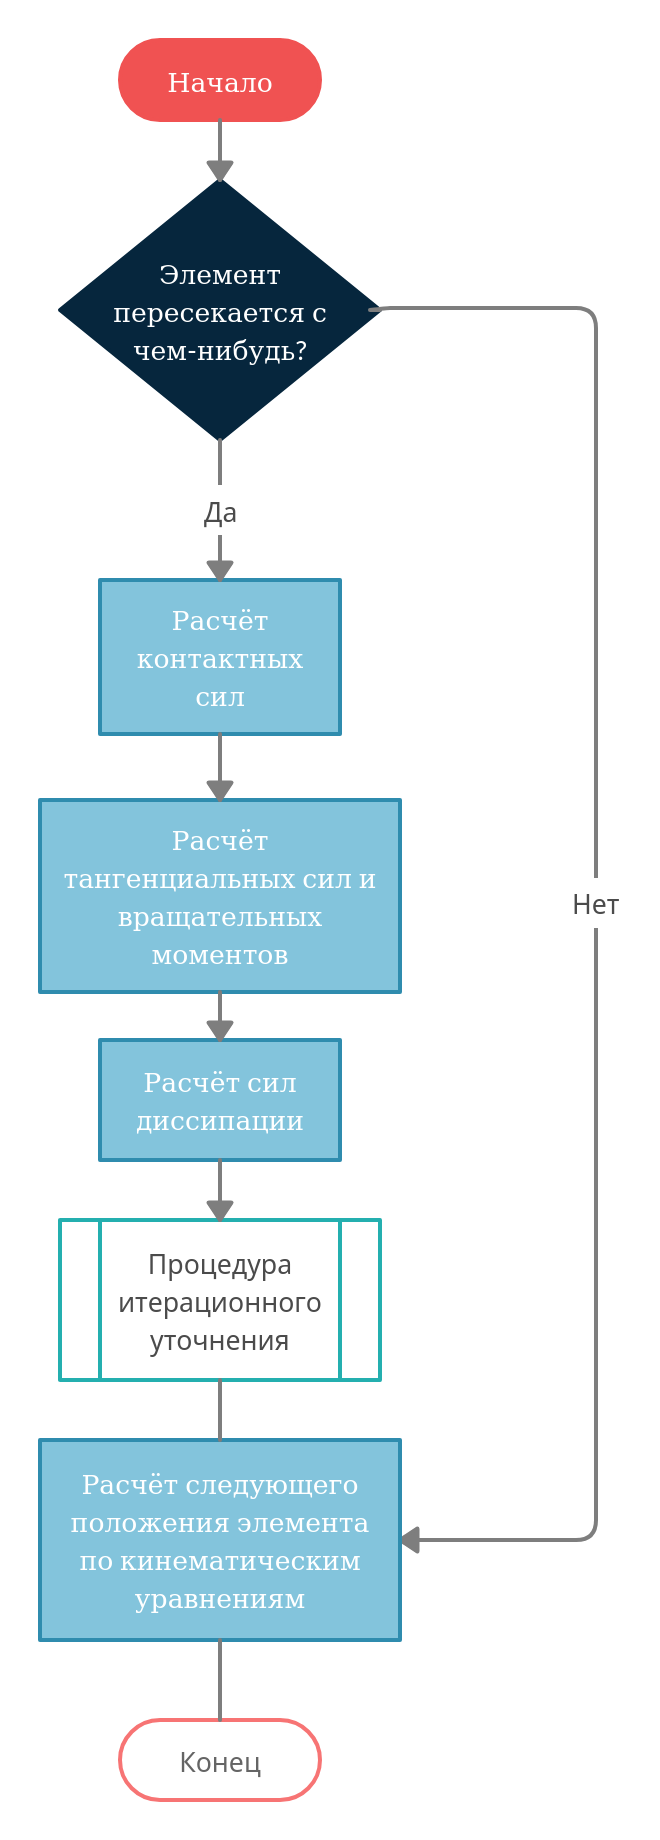
\includegraphics[width=0.5\textwidth]{big_block}
	\caption{Блок-схема работы алгоритма на одном шаге}
	\label{pic:osn_block}
\end{figure} 

В двойном цикле проходимся по каждому возможному сочетанию шаров и проверяем пересекаются ли они.
Если нет -- проверяем следующую возможную пару.
Если да -- необходимо перейти в локальную систему координат, связанную с положением шаров в пространстве друг относительно друга. Все величины, необходимые для расчёта (скорость, ускорение и пр.), переводятся в данную систему координат.

\begin{figure}[H]
	\centering
	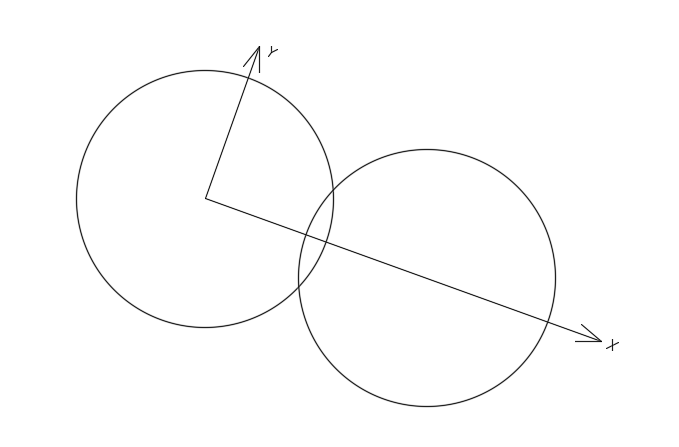
\includegraphics[width=0.5\textwidth]{local}
	\caption{Демонстрация локальной системы координат}
	\label{pic:local}
\end{figure} 

Далее необходимо рассчитать силовые факторы, действующие на шар: силы контактного взаимодействия (по алгоритму \ref{force_subsection}), силы диссипации (по алгоритму \ref{dempf_subsection}), моменты в плоскости (по алгоритму \ref{angular_subsection}). 
Нужно также не забыть учесть для каждого из шаров силы удалённого действия которые считаются в каждый момент времени (в нашей модели это будет поле ускорений (пункт \ref{dempf_subsection})). 
После нахождения сочетания сил действующих на тело проводится итерационная процедура уточнения (описанная в \ref{iter_subsection})

Когда говорится о каждом возможном сочетании шаров имеется в виду также взаимодействие со стенкой, которой ограничено движение шара. 
В данной работе подробный алгоритм взаимодействия со стенкой описывался в пункте \ref{wall_subsection}.

Итого, второй закон Ньютона при взаимодействии шара с другими объектами имеет следующий вид
\begin{align}
\overline{m \cdot a} &= \overline{F_n} + \overline{F_s} + \overline{D} + \overline{G}\\
\overline{I \cdot \varepsilon} &= \overline{M_s} + \overline{M_r}
\end{align}

где $m$ --- масса элемента, [кг];

$\overline{a}$ --- вектор линейного ускорения элемента от данного взаимодействия, [Н / кг];

$\overline{F_n}$ --- вектор контактной силы, действующий в направлении нормали данного взаимодействия, [Н];

$\overline{F_s}$ --- вектор силы трения скольжения данного взаимодействия, [Н];

$ \overline{D}$ --- вектор сил диссипации, действующих на элемент в результате данного взаимодействия, [Н];

$\overline{G}$ --- вектор сил удалённого действия, действующих на элемент все время, [Н];

$I$ --- момент инерции данного элемента относительно центра, [кг $ \cdot $ м$^2$];

$ \overline{\varepsilon}$ --- вектор углового ускорения элемента от данного взаимодействия, [1 / с$^2$];

$ \overline{M_s}$ --- вектор момента, возникающий в результате приведения силы трения скольжения в центр (механизм будет показан в следующих пунктах), [Н $ \cdot $ м];

$\overline{M_r}$ --- вектор момента трения качения данного взаимодействия, [Н $ \cdot $ м];
\\

После -- необходим переход в глобальную систему координат.

После расчёта и уточнения всех сил производится интегрирование -- расчёт нового положения каждого из шаров, в соответствии с законами кинематики.

Можем довольно легко оценить сложность этого алгоритма: время -- $O(n^2)$, память $O(n)$. 
Безусловно для большого числа элементов (от 100) данная задача осложняется существенной вычислительной емкостью.
Путей решения данной проблемы два.
Первый -- использование хэширования. 
Деление пространства на определённые участки и проверка пересечения шаров не со всеми шарами, а только с близлежащими участками.
При правильном выборе сетки, которой покрывается пространство это позволит уменьшить сложность по времени до $O(n)$.

Второй путь решения данной проблемы -- распараллеливание процессов подсчёта на одном шаге разных независимых участков пространство (необходимо сначала будет реализовать первый подход). Это сможет увеличить время подсчёта лишь на константу, но эта константа будет тем больше, чем больше шаров участвует в моделировании.




\subsection{Кинематика частиц}
\label{kinem_subsection}

В данной работе рассматривается элемент с тремя степенями свободы: 2-мя линейными и 1-ой угловой.
В декартовой системе координат они обозначаются как $x$, $y$ и $\vartheta$.
В локальной системе координат эти степени свободы имеют следующие обозначения как $n$, $t$ и $\vartheta$. Соответственно направление нормали к взаимодействию, тангенциальное направление и угловое (не изменяется от перехода от глобальной системы координат к локальной).

Кинематические уравнения для расчёта нового положения тела на шаге могут быть представлены следующим образом
\begin{align}
x &= x_0 + v^x_0 \cdot \Delta t + \dfrac{a^x_0 \cdot \Delta t^2}{2} + \dfrac{b^x_0 \cdot \Delta t^3}{6}\\
y &= y_0 + v^y_0 \cdot \Delta t + \dfrac{a^y_0 \cdot \Delta t^2}{2} + \dfrac{b^y_0 \cdot \Delta t^3}{6}\\
\vartheta &= \vartheta_0 + v^{\vartheta}_0 \cdot \Delta t + \dfrac{a^{\vartheta}_0 \cdot \Delta t^2}{2} + \dfrac{b^{\vartheta}_0 \cdot \Delta t^3}{6}
\end{align}

\begin{align}
v^x &= v^x_0 + a^x_0 \cdot \Delta t + \dfrac{b^x_0 \cdot \Delta t^2}{2}\\
v^y &= v^y_0 + a^y_0 \cdot \Delta t + \dfrac{b^y_0 \cdot \Delta t^2}{2}\\
v^{\vartheta} &= v^{\vartheta}_0 + a^{\vartheta}_0 \cdot \Delta t + \dfrac{b^{\vartheta}_0 \cdot \Delta t^2}{2}
\end{align}


$b_0^i$ в данных уравнения -- рывок по $i$-той координате. 
Его значение получается в результате итерационного процесса.
Конкретно данная процедура будет обсуждаться в пункте \ref{iter_subsection}.



\subsection{Расчёт контактных сил}
\label{force_subsection}

\textit{Силы в нормальном направлении.}

Контактная сила шаров при их пересечении будет определяться как
\begin{equation}
\label{norm_force}
F_n = k_n \cdot \delta_n
\end{equation}

где $F_n$ --- контактная сила, возникающая в точке контакта и действующая на оба шара, [Н];

$k_n$ --- коэффициент жёсткости, [Н/м];

$\delta_n$ --- взаимное проникновение, так называемое вхождение шаров друг в друга, [м].

При построении модели расчёта сил при взаимодействии элементов друг с другом необходимо определиться с выбором построения модели жёсткости. 
Cundall в своей работе \cite{cundall} описывал постоянную жёсткость, которая зависит исключительно от свойств материала.
\begin{equation}
\label{kn_const}
k_n = const
\end{equation}


Как альтернатива, существует упрощённое решение контактной задачи Герца \cite{friction_calibration}.
Оно используется наиболее часто при моделирование процессов МДЭ.
Исходя из него жёсткость зависит и от свойств материала, и от вхождения, и от радиусов шаров:

\begin{equation}
\label{kn_herz}
k_n = \frac{4}{3} \cdot E_{eff} \cdot \sqrt{R_{eff} \cdot \delta_n}
\end{equation}
где 
\begin{align}
\dfrac{1}{E_{eff}} = \dfrac{1 - \nu_1^2}{E_1} + \dfrac{1 - \nu_2^2}{E_2} \qquad \qquad \qquad \dfrac{1}{R_{eff}} = \dfrac{1}{R_1} + \dfrac{1}{R_2}
\end{align}


В дальнейшей работе программы будет выбрана модель Герца.


\textit{Крутящие силовые факторы и силы в тангенциальном направлении}
\label{angular_subsection}


В процессе взаимодействия двух шаров помимо силы в нормальном направлении из-за коэффициентов трения появляются сила в тангенциальном направлении и момент.

\begin{figure}[H]
	\centering
	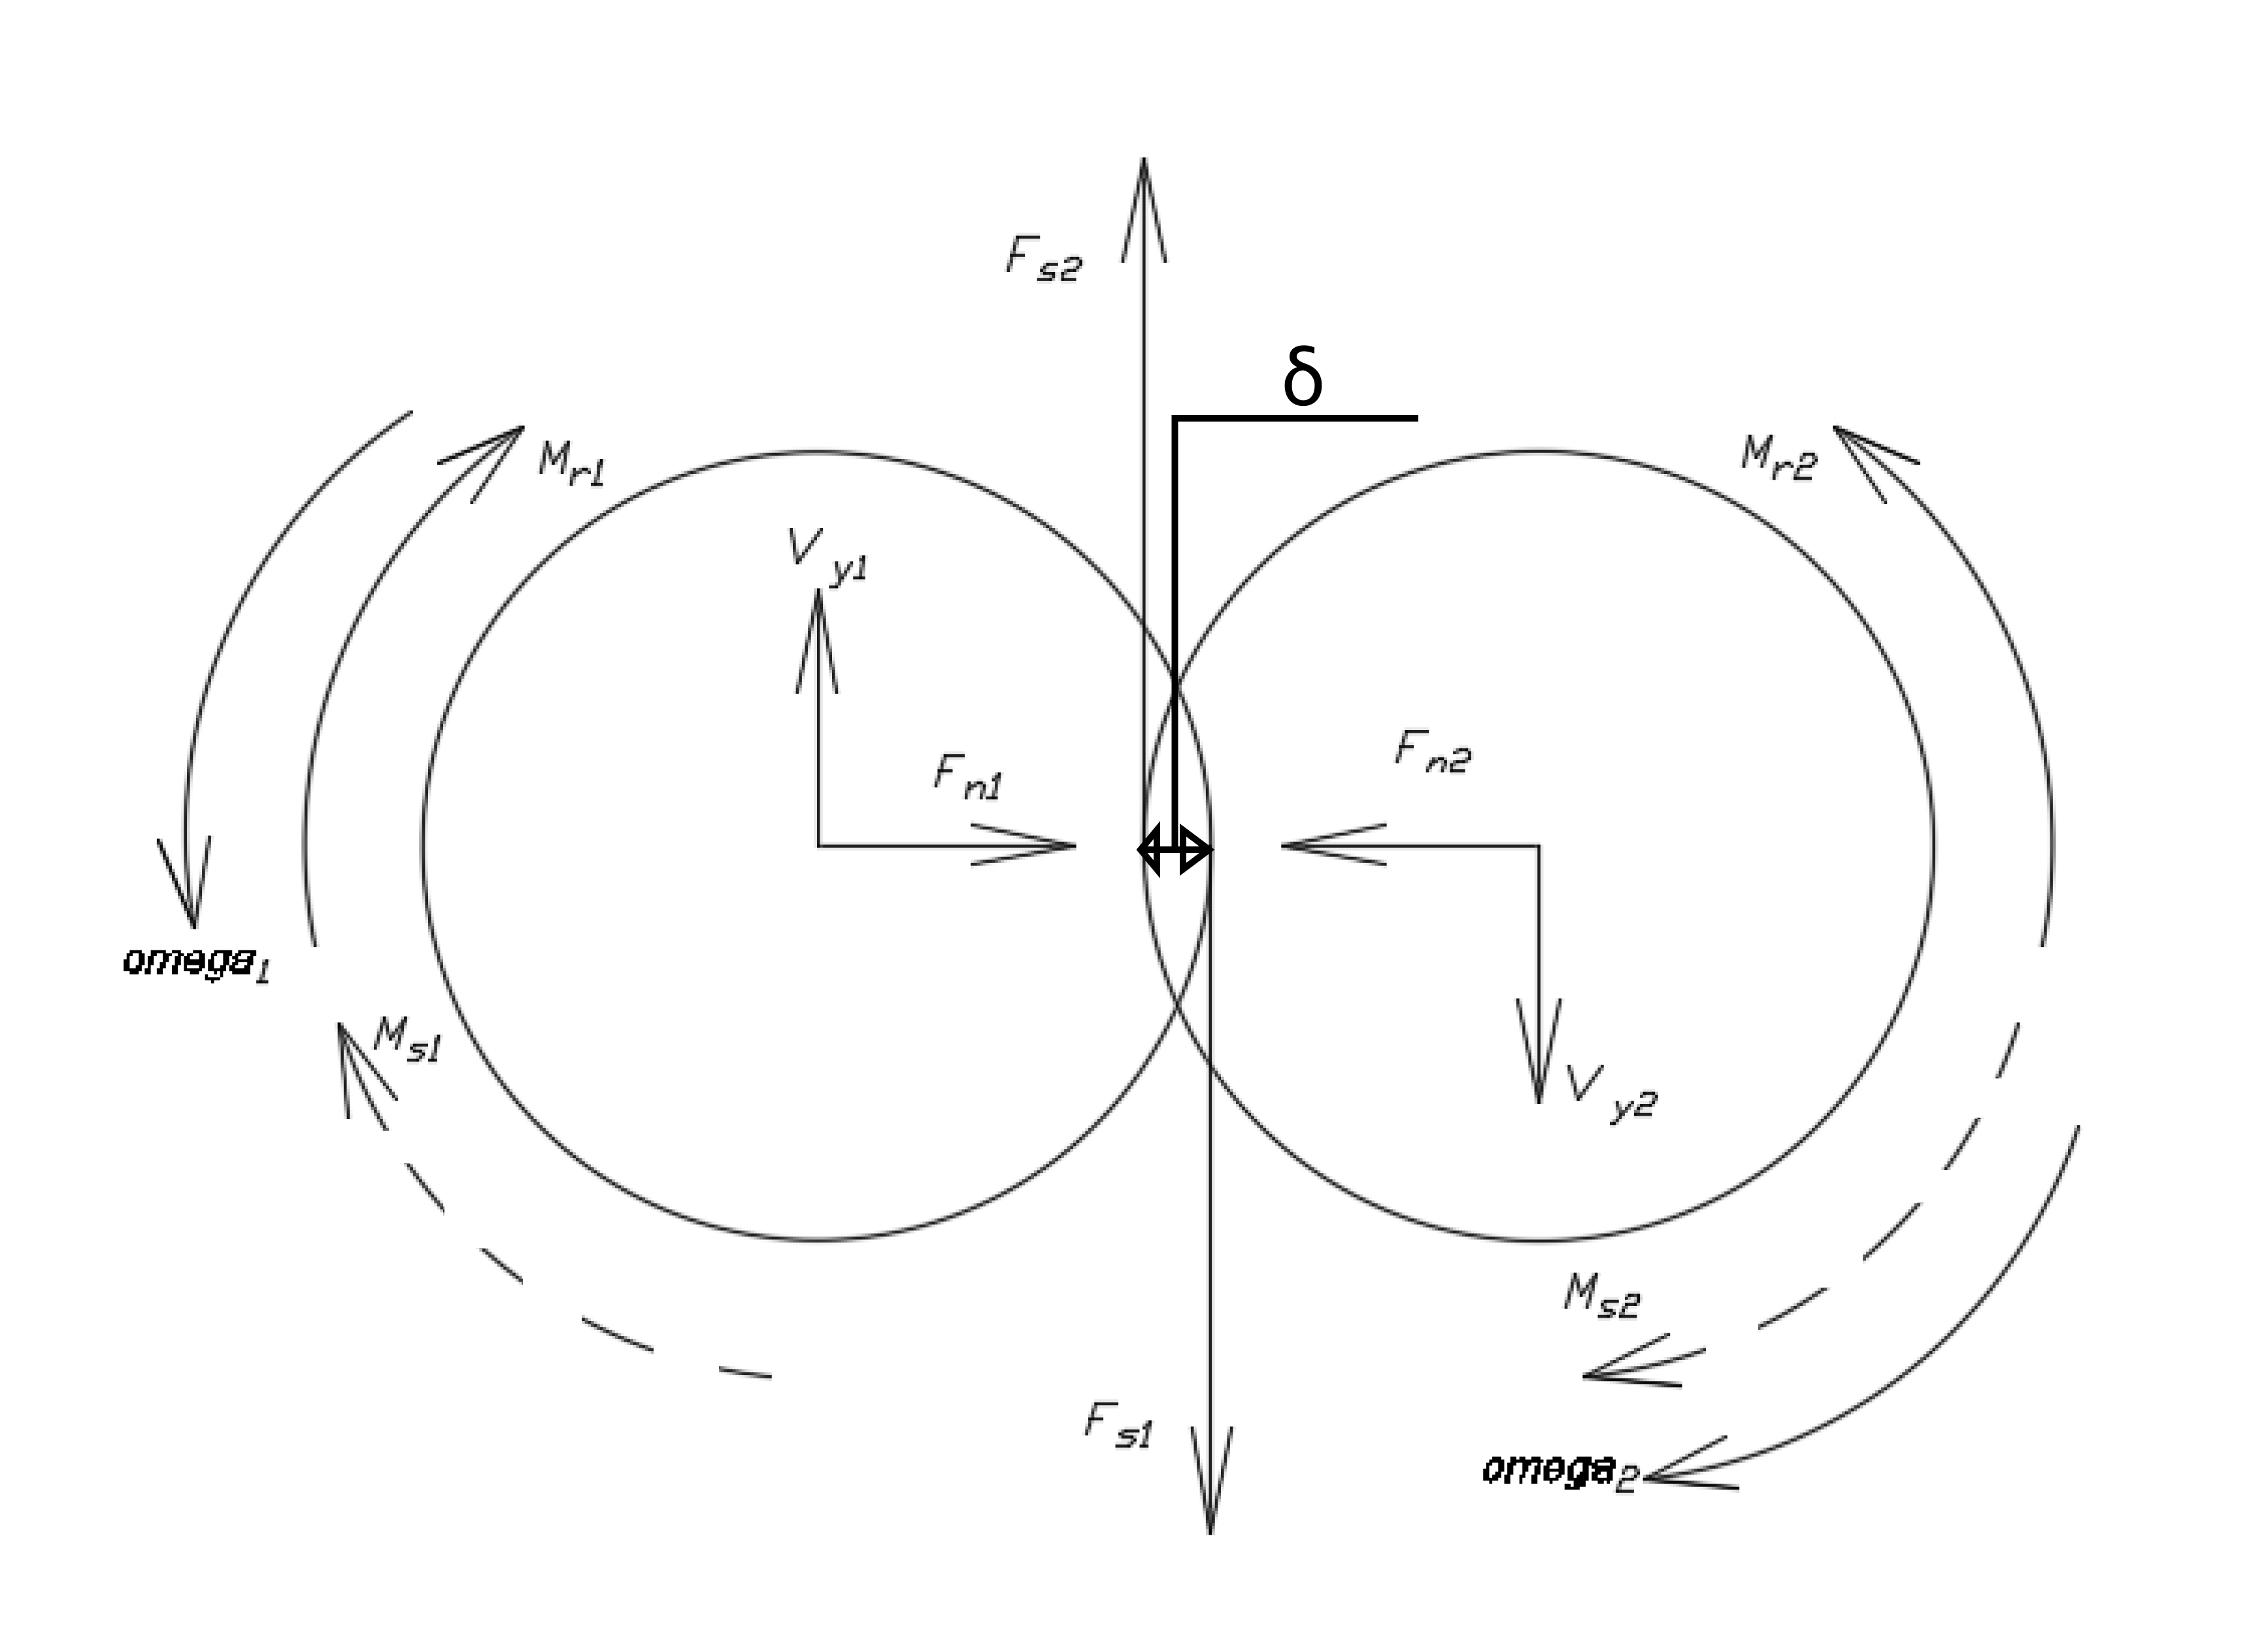
\includegraphics[width=0.8\textwidth]{sily}
	\caption{Силы возникающие в шарах при контактном взаимодействии.}
	\label{pic:sily}
\end{figure} 

Сила в тангенциальном направлении будет появляться из-за трения скольжения и направлена в противоположном относительной тангенциальной скорости шара в точке контакта (относительно другого шара) \cite{friction_calibration}. На рисунке \ref{pic:sily} сила скольжения обозначена $F_s$. Сила скольжения определяется по формуле
\begin{align}
\label{sliding_force}
F_s = \mu_s \cdot F_n \cdot sign(v_{rel\_tan}) \qquad \qquad \qquad v_{rel\_tan} \neq 0
\end{align}

где $\mu_s$ --- безразмерный коэффициент трения скольжения (зависит только от свойств материала);

$F_n$ --- контактная сила действующая на элемент в нормальном направлении, [Н];

$v_{rel\_tan}$ --- тангенциальная скорость шара в точке контакта, относительно другого шара, [м/с].


Отдельного обсуждения стоит расчёт относительной тангенциальной скорости шара. 
Помимо тангенциальной скорости центра шара ($v_y$ на рисунке \ref{pic:sily}) в относительную тангенциальную скорость в точке контакта также будет входить угловая скорость домноженная на радиус шара.
Итого, формула для определения $v_{rel\_tan}$ выглядит следующим образом (верхним индексом обозначены номера шаров: 1 -- шар для которого проводится расчёт, 2 -- шар, вступивший с ним в контакт):
\begin{align}
\label{rel_tan_velocity}
v_{rel\_tan}^{1} = v_{y}^{1} - v_{y}^{2} - \left( \omega_1 \cdot R_1 + \omega_2 \cdot R_2 \right)
\end{align}

\begin{figure}[H]
	\centering
	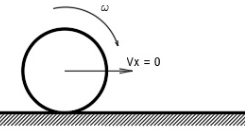
\includegraphics[width=0.5\textwidth]{pol_omega}
	\caption{Шар должен катится по неабсолютно гладкому полу при ненулевой угловой скорости и нулевой линейной.}
	\label{pic:pol_omega}
\end{figure} 

Помимо понятного с точки зрения физического смысла объяснения необходимости учёта добавка угловой скорости можно привести следующий пример. 
Если вращающийся вокруг оси параллельной полу шар (не имеющий линейной скорости) поставить на этот пол, то шар обретёт линейную скорость и покатится (рисунок \ref{pic:pol_omega}). 
Этот эффект объясняется наличием силы трения скольжения и этого самого добавка.

\begin{figure}[H]
	\centering
	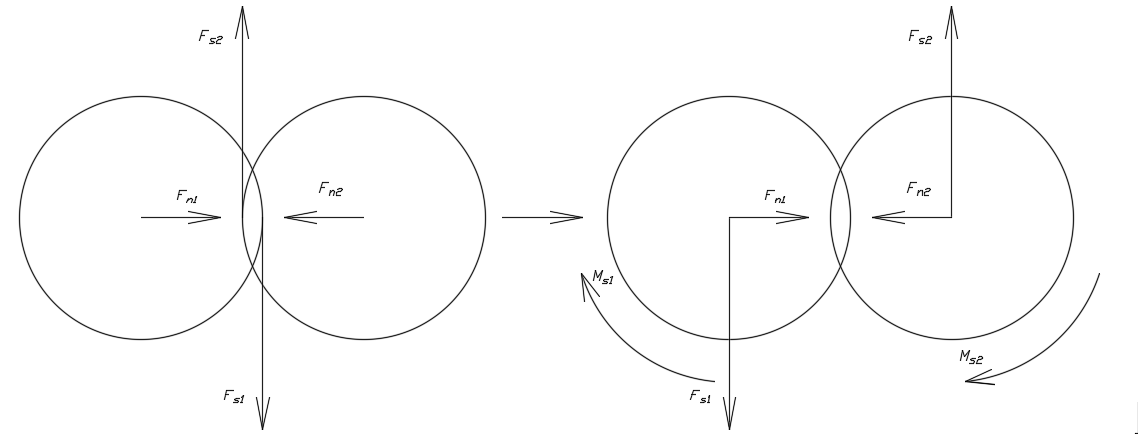
\includegraphics[width=0.8\textwidth]{fs_ms}
	\caption{Приведение силы трения скольжения к центру элемента}
	\label{pic:fs_ms}
\end{figure} 

\begin{align}
\label{sliding_moment}
M_s = F_s \cdot R_{eff}
\end{align}

\[
\text{где} \quad \dfrac{1}{R_{eff}} = \dfrac{1}{R_1} + \dfrac{1}{R_2} \quad \text{ --- эффективный радиус, [м]}
\]

Из-за того что сила $F_s$ действует в точке контакта при переносе её в центр тяжести от неё появляется момент $M_s$, который определяется по формуле ниже с учётом знака перевода из линейной координаты в угловую (рисунок \ref{pic:fs_ms}).



Момент $M_r$ же появляется из-за трения качения и определяется следующим образом.

\begin{align}
\label{rolling_moment}
M_r = \mu_r \cdot F_n \cdot R_{eff} \cdot sign(\omega_{rel}) \qquad \qquad \qquad \omega_{rel} \neq 0
\end{align}

где $\mu_r$ --- безразмерный коэффициент трения качения (зависит только от свойств материала);

$\omega_{rel}$ --- угловая скорость шара, относительно другого шара, [рад/с].

Т.к. $\omega_{rel}$ относительная угловая скорость при внешнем зацеплении шаров она считается по формуле 
\begin{align}
\label{omega_rel}
\omega_{rel} = \omega_1 + \omega_2
\end{align}

В этих формулах вводится эффективный радиус из следующих соображений: если домножать силу на обычный радиус, то на каждом моменте $t$ данного расчёта мы не можем говорить о выполнении второго закона Ньютона (при разных радиусах контактирующих шаров моменты $M_s$ и $M_r$ будут разные по модулю на шарах, участвующих в контакте).
Эффективный радиус же позволяет добиться равенства моментов, действующих на два контактирующих тела, в каждый момент времени.


\subsection{Диссипация}
\label{dempf_subsection}

Силы диссипации возникают, потому что контактное взаимодействие двух шаров воспринимают как пружину с демпфером (рисунок \ref{pic:dempf}) \cite{pruzhina}. 
Энергия сжатой пружины также будет учитываться далее и записываться как потенциальная.

\begin{equation}
\label{eq:pot_energy}
E_{pot} = \dfrac{k \cdot \delta^2}{2}
\end{equation}


где $E_{pot}$ --- энергия сжатия пружины, [Дж];

$k$ --- жёсткость пружины, [Н / м];

$\delta$ --- проникновение шаров друг в друга в направлении нормали, [м].

\begin{figure}[H]
	\centering
	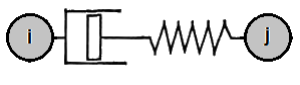
\includegraphics[width=0.4\textwidth]{dempf}
	\caption{При контактном взаимодействии связь шаров можно представить в виде пружины и демпфера.}
	\label{pic:dempf}
\end{figure} 

Силы диссипации линейно зависят от относительной скорости и действуют в противоположном направлении.
Относительная скорость для каждого шара считается в направлении нормали.
Нормалью  далее будем называть направление от центра шара до центра шара, с которым он контактирует.
\begin{equation}
\label{dempf_force}
D_n = c_n \cdot v_n
\end{equation}

где $D_n$ --- сила диссипации в нормальном направлении, [Н];

$c_n$ --- коэффициент диссипации в нормальном направлении, [(Н $\cdot$ с) / м];

$v_n$ --- относительная скорость движения шаров в нормальном направлении, [м / с].

Как и силы гравитации в численном методе силы диссипации будут суммироваться и использоваться для расчёта положения, скорости и ускорения тела на очередном шаге.

Аналогично, диссипация считается в тангенциальном направлении \cite{many_pruzhina}.
\begin{equation}
\label{dempf_force_tangent}
D_t = c_t \cdot v_t
\end{equation}

где $D_t$ --- сила диссипации в тангенциальном направлении, [Н];

$c_t$ --- коэффициент диссипации в тангенциальном направлении, [(Н $\cdot$ с) / м];

$v_t$ --- относительная скорость движения шаров в тангенциальном направлении, [м / с].

Относительная скорость в нормальном направлении определяется как
\begin{equation}
v_n = v_n^1 - v_n^2
\end{equation}
Относительная скорость в тангенциальном направлении же определяется по формуле \ref{rel_tan_velocity}.

По контактной модели Герца \cite{aglomerath} коэффициенты диссипации непостоянны и зависят не только от обработки элементов и свойств материала, но и от размеров контактирующих шаров и их вхождений друг в друга.
\begin{align}
\label{kef_dempf}
c_n &= 2 \cdot \sqrt{m \cdot 2 \cdot E_{eff} \cdot \delta_n \sqrt{R_{eff}}} \cdot \zeta_n \\
c_t &= 4 \cdot \sqrt{m \cdot 2 \cdot G_{eff} \cdot \delta_n \sqrt{R_{eff}}} \cdot \zeta_t
\end{align}

Стоит также упомянуть о силах поля.
В качестве сил удалённого действия в данной работе выступает только гравитация.
Соответственно
\begin{align}
G^x &= 0 \\
G^y &= m \cdot 9.81
\end{align}
На угловую координату силы поля действовать никак не будут.

\subsection{Частный случай взаимодействия шар-стена}
\label{wall_subsection}

\begin{figure}[H]
	\centering
	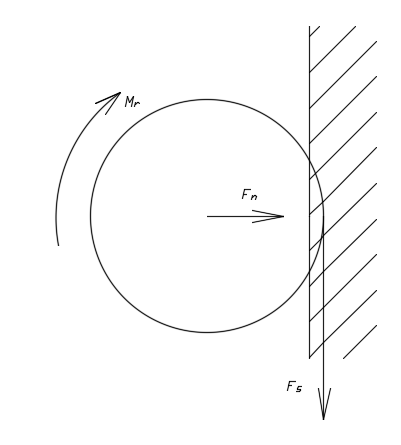
\includegraphics[width=0.5\textwidth]{ball_wall}
	\caption{Взаимодействие шара со стоеной}
	\label{pic:ball_wall}
\end{figure} 

Элементы в данной модели ограничены стенкой. 
Поэтому необходимо рассмотреть взаимодействие элемент-стена.
Это можно считать частным случаем описанного выше алгоритма с несколькими отличительными чертами.

1) Стенка представлена как замкнутая фигура, состоящая из конечного числа прямых линий.

2) Шар никак не влияет на стенку. 
Её движение зависит только от заданного ей закона движения.

3) При расчёте сил трения используется не эффективный радиус, а радиус данного шара.

4) Стенка вращается относительно какой-то точки.
В данной модели это будет геометрический центр стенки.
Так же важно упомянуть об угловом направлении при вращении стенки.
Если при взаимодействии шаров мы говорили о внешнем зацеплении, то здесь уместно рассматривать внутреннее зацепление шара со стенкой (термин аналогичен зацеплению шестеренок в задачах теоретической механики).
Следовательно в формулах \ref{omega_rel} и \ref{rel_tan_velocity} угловая скорость стенки будет идти со знаком минус.


 
\subsection{Итерационное уточнение}
\label{iter_subsection}

%В качестве численного интегрирования в данной работе используется метод прямоугольников (это выходит из принципа 1 упрощений МДЭ).

Интегрирование в данной задаче можно было бы назвать точным, а не численным, если бы задача была линейной.
Но данная задача является нелинейной. 
Если на момент начала шага по времени $t$ на тело действует сила $F_t$, то на момент начала следующего шага по времени $t + \Delta t$ уже будет действовать сила $F_{t + \Delta t}$, которая будет другой и зависеть от величины вхождения шаров друг в друга на момент конца текущего шага по времени, и, следовательно, от закона движения частиц за шаг по времени. 
Закон изменения силы заранее неизвестен.

На первой итерации решения мы принимаем закон изменения сил постоянным (первое приближение к значению силы на конце шага).
Начиная со второй итерации примем изменение силы линейным на участке от $t$ до $t + \Delta t$  и тогда для интегрирования необходимо ввести ещё один член, который называется рывок. 
Рывок характеризует изменение ускорения.
Обозначим рывок $b_n$.
Тогда
\begin{align}
a_{t + \Delta t} &= a_t + b_n \cdot \Delta t \\
v_{t + \Delta t} &= v_t + a_t \cdot \Delta t + \dfrac{b_n \cdot \Delta t^2}{2} \\
x_{t + \Delta t} &= x_t + v_t \cdot \Delta t + \dfrac{a_t \cdot \Delta t^2}{2} +  \dfrac{b_n \cdot \Delta t^3}{6}
\end{align}

Сам по себе рывок можно рассчитать как
\begin{align}
\label{jerk_normal}
b_n = \dfrac{a_{t + \Delta t} - a_{t}}{\Delta t}
\end{align}

Но пока мы не оказались в начале следующего шага $a_{t + \Delta t}$ нам не известен.
Поэтому для расчёта рывка проводится итерационный процесс. 
В начале каждого шага $t$ проводится расчёт изменения вхождения $\Delta \delta = \delta_{t + \Delta t} - \delta_t$ по следующей формуле
\begin{align}
\Delta \delta = v_t \cdot \Delta t + \dfrac{a_t \cdot \Delta t^2}{2} +  \dfrac{b_n \cdot \Delta t^3}{6}
\end{align}

В первую итерацию цикла $b_n$ принимается равным нулю.
Отсюда можем получить перекрытие на начало следующего шага $\delta_{t + \Delta t} = \delta_t + \Delta \delta$.
Далее по закону зависимости \ref{norm_force} необходимо найти силу в начале следующего шага $F_{t + \Delta t}$ и ускорение $a_{t + \Delta t}$.

Следующим действием нужно проверить удовлетворяет ли нас $a_{t + \Delta t}$ и если нет -- начать итерационную процедуру заново.
Проверкой того что $a_{t + \Delta t}$ нас удовлетворяет и его не надо уточнять (то есть условием выхода из цикла) является критерий выхода из цикла по ускорению.
Это значит, что $a_{t + \Delta t}^k$ должно незначительно отличаться от  $a_{t + \Delta t}^{k-1}$ (верхним индексом отмечен номер итерации на начало шага $t$):
\begin{equation}
\label{jerk_condition}
\left| \dfrac{a_{t + \Delta t}^k - a_{t + \Delta t}^{k-1}}{a_{t + \Delta t}^k} \right| < \varepsilon_a
\end{equation}

После нахождения $a_{t + \Delta t}$ по формуле \ref{jerk_normal} можем найти рывок $b$.

Данный процесс показан для нахождения рывка в направлении нормали (понятие нормали было введено в разделе введения  диссипации \ref{dempf_subsection}). 
Процесс нахождения рывков в тангенциальном и угловом направлениях не сильно отличается от указанного выше.

На каждой итерации после нахождения части нормальной контактной силы $\Delta F = F_{t+\Delta t} - F_t$  мы можем найти $\Delta F_s$, $\Delta M_s$, $\Delta M_r$ по формулам \ref{sliding_force}, \ref{sliding_moment} и \ref{rolling_moment}, соответственно.
Аналогично формуле \ref{jerk_normal} находим рывки в тангенциальном и угловом направлениях.
\begin{align}
b_t &= \dfrac{a_{t + \Delta t} - a_{t}}{\Delta t} \label{jerk_tangent}\\
b_{\vartheta} &= \dfrac{\varepsilon_{t + \Delta t} - \varepsilon_{t}}{\Delta t} \label{jerk_angular}
\end{align}

В таком случае условием выхода из цикла будет удовлетворение условию \ref{jerk_condition} для всех трёх направлений одновременно.

Блок-схема данного процесса представлена на рисунке \ref{pic:iter}.

\begin{figure}[H]
	\centering
	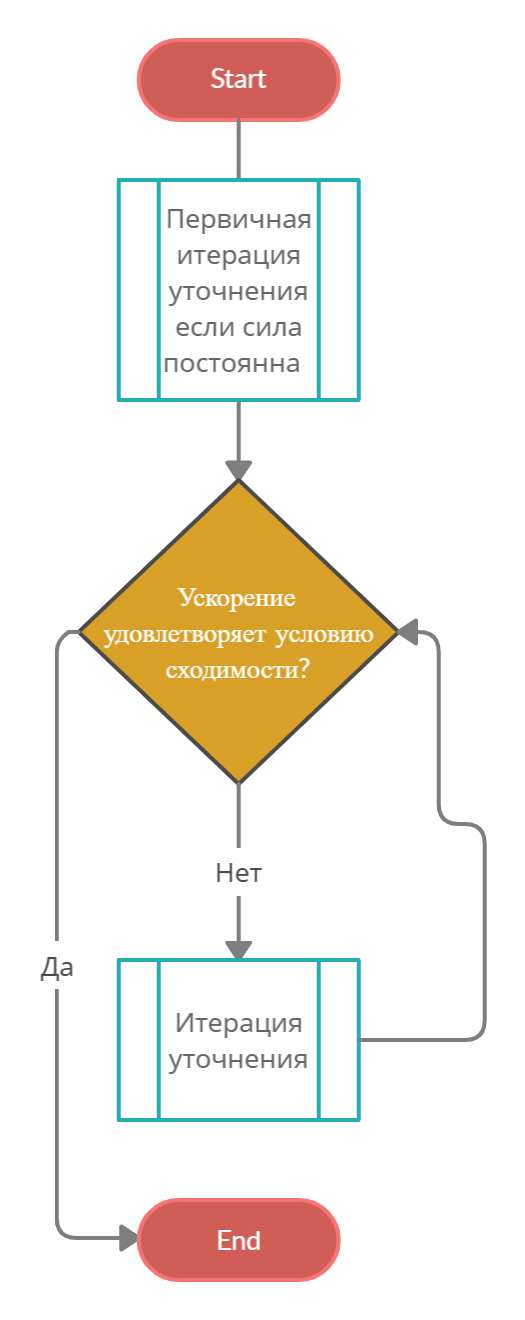
\includegraphics[width=0.4\textwidth]{iter_cicle} 
	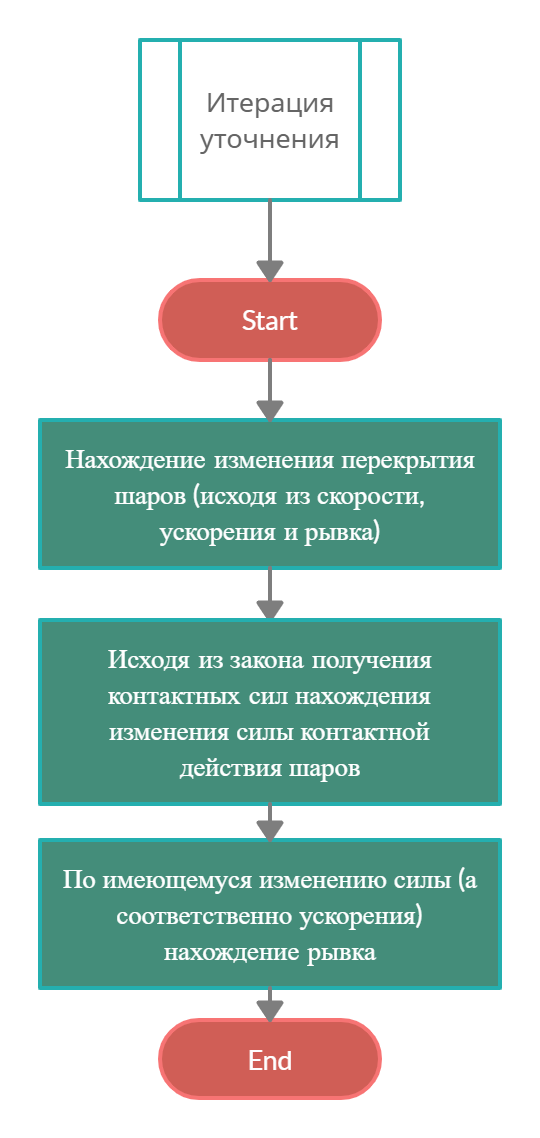
\includegraphics[width=0.4\textwidth]{iter_one}
	\caption{Блок-схема итерационного процесса: слева цикл и условие выхода, справа -- сама процедура уточнения (одна итерация)}
	\label{pic:iter}
\end{figure} 

\subsection{Модель разрушения}
\label{sub:break_model}
Для моделирования работы необходимо задаться моделью разрушения.
Выберем энергетический способ, описанный в \cite{razr}.

Для каждой частицы, находящейся в контакте с другими частицами и/или геометрическими поверхностями, рассчитывается общая удельная энергия $E_t$ контакта.
Если эта энергия больше, чем минимальная энергия разрушения частицы ($E_{min}$, которая является константой материала), то $E_{t}$ определяется как
\begin{equation}
\label{eq:break_Et}
E_t = E_{cum} + E - E_{min}
\end{equation}

где $E_{cum}$ -- накопленная энергия предыдущих контактов (в начальный момент времени равна 0), $E$ -- текущая энергия контакта, которая определяется в формуле \ref{eq:pot_energy} и появляется только в следствие упругого взаимодействия частиц.
\begin{equation}
\label{eq:break_E}
E = \frac{k \cdot \delta^2}{2}
\end{equation}

Вероятность разрушения частиц рассчитывается по формуле
\begin{equation}
\label{eq:break_P}
P = 1 - e^{-S \cdot E_t} 
\end{equation}
где $S$ — параметр прочности, характеризующий разрушение частиц. Данная формула является эмпирической, коэффициенты подбираются для каждого типа руды по отдельности на основе экспериментальных данных о разрушении.


Если частица разрушена, то ее фрагменты (тоже формы шара) генерируются исходя из равенства массы и равенства кинетической энергии. 
Т.к. в данной работе рассматривается работа в двухмерном пространстве, то сохранение массы шара, хоть и сопровождается сохранением площади в трехмерном пространстве, в нашей постановке вызовет "проблему наложения". 
Будет происходить зрительное увеличение занимаемой площади шаров.
Например, образуется две новых частицы.
Тогда исходя из равенства мссс новый радиус расчитывается как
\begin{equation*}
R_{old}^3 = 2 \cdot R^3_{new} \qquad \rightarrow \qquad R_{new} =\frac{R_{old}}{\sqrt[3]{2}}
\end{equation*}
Но когда частицы будут отрисовываться, то они будут занимать больше места.
\begin{equation*}
S_{old} = \frac{\pi \cdot R_{old}^2}{2} \qquad \qquad S_{new} = 2 \cdot \frac{\pi \cdot R_{new}^2}{2} = \sqrt[3]{2} \cdot \frac{\pi \cdot R_{old}^2}{2} = \sqrt[3]{2} \cdot S_{old}
\end{equation*}
При увеличении количества частиц $S_{new}$ будет стремиться к $S_{old}$.
\begin{figure}[H]
	\centering
	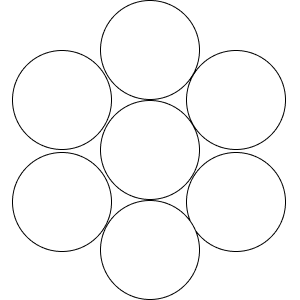
\includegraphics[width=0.5\textwidth]{1_balls} 
	\caption{Шары до разрушения}
	\label{pic:1_balls}
\end{figure} 
В данной реализации для решения вопроса пространства шарам будет разрешено пересекаться с другими без воздействия сил друг на друга, если в первый момент своего появления они уже с кем-то перескаются.
Иначе частицы в самый первый момент будут сильно накладываться друг на друга и между ними будут образовываться слишком большие силы отталкивания, чего быть не должно.
После потери первичного контакта все частицы начинают полноценно взаимодействовать друг с другом.
Это не повлияет качественно на работу программы.
Ниже на рисунках \ref{pic:2_balls} -- \ref{pic:4_balls} представлены ситуации разбиения шаров на n элементов.
\begin{figure}[H]
	\centering
	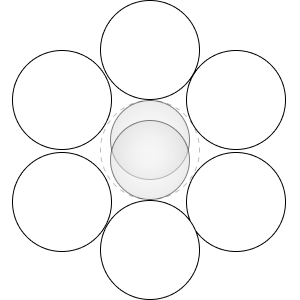
\includegraphics[width=0.5\textwidth]{2_balls} 
	\caption{Случай разлета шара на 2 частицы}
	\label{pic:2_balls}
\end{figure} 

\begin{figure}[H]
	\centering
	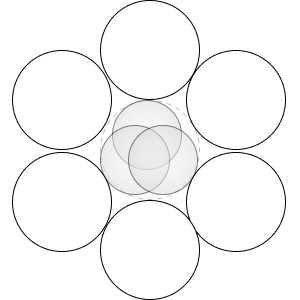
\includegraphics[width=0.5\textwidth]{3_balls} 
	\caption{Случай разлета шара на 3 частицы}
	\label{pic:3_balls}
\end{figure} 

\begin{figure}[H]
	\centering
	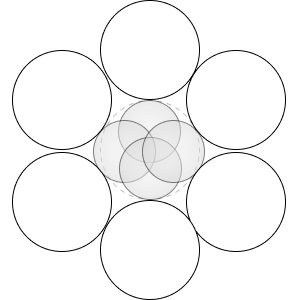
\includegraphics[width=0.5\textwidth]{4_balls} 
	\caption{Случай разлета шара на 4 частицы}
	\label{pic:4_balls}
\end{figure} 


При разломе шара, количество сгенерированных частиц образуется исходя из нормального распределения с математическим ожиданием $3\sigma$ и медианой 4, таким образом чтобы 99.7\% величин лежало между двумя и шестью частицами.

Из вышесказанного становится ясно, что наибольшее воздействие на частицу и на вероятность ее разрушения будет оказывать ударное взаимодействие.
Только достаточно большая энергия от удара будет влиять на вероятность разрушения, а энергия в свою очередь зависит от величины проникновения одного шара в другой.
Величина же проникновения будет максимальной когда относительная скорость движения шаров друг на встречу другу максимальна. Что и называется ударным взаимодействием.



\subsection{Анализ и проверка адекватности существующей модели}

В качестве проверки адекватности построения данной модели, а также проверки ошибок в решении были использованы несколько различных подходов.

1) Для проверки физичности и логичности результатов использовалось отображение положения и движения шаров.
При прорисовке, например, каждого сотого или тысячного кадра это не так заметно сказывалось на скорости работы программы (время одной прорисовки мало по сравнению с расчётом ста шагов N-го количества шаров), но позволяло оценить корректность и найти логические ошибки на самых ранних стадиях построения решения.

2) Для проверки энергетической составляющей работы алгоритма (а также для корректности диссипирующей модели) использовались графики изменения энергии всей системы во времени (при нулевой диссипации энергия должна быть неизменной, при ненулевой -- энергия должна падать, а система приходить к состоянию равновесия) (рисунок \ref{pic:graphs}) и графики изменения скорости и контактной силы (рисунок \ref{pic:graphs}). Нижеприведенные графики являются примером и не могут быть проанализированы вне контекста.


\begin{figure}[H]
	\centering
	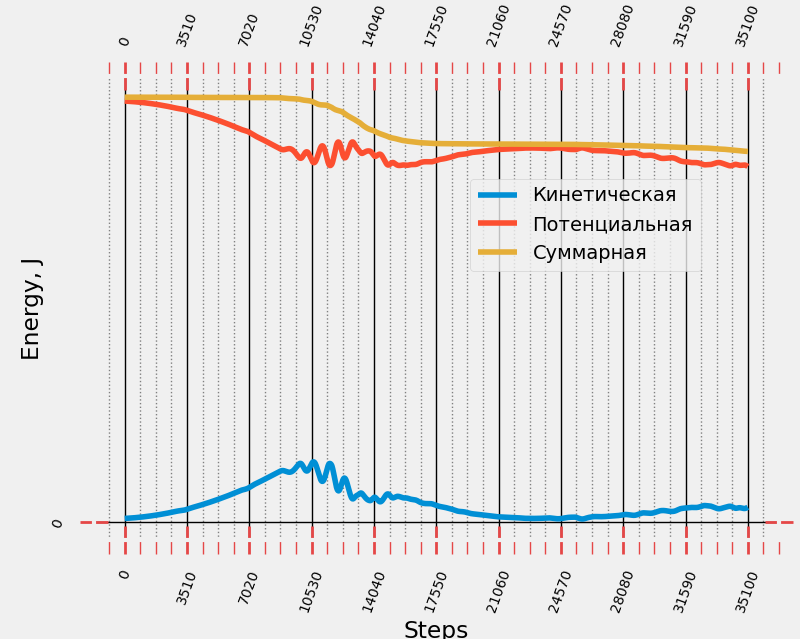
\includegraphics[width=0.4\textwidth , height=0.25\textheight]{graph1} 
	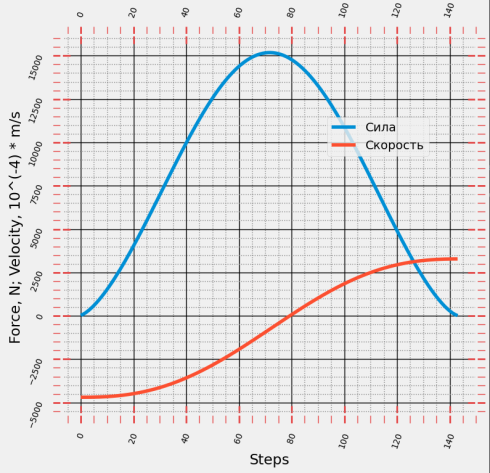
\includegraphics[width=0.4\textwidth , height=0.25\textheight]{graph2}
	\caption{Графики зависимости энергии, силы и скорости}
	\label{pic:graphs}
\end{figure} 

3) Для проверки корректности вращательных модели был проведён ряд тривиальных тестов (около 20 штук), для каждого из которых можно было провести простые аналитические расчеты. 
Проверялись корректность направления возникающих сил, моментов и скоростей при различных ситуациях (два шара с нулевой линейной скоростью и ненулевой угловой контактируют, два шара с нулевой угловой скоростью и ненулевой линейной контактируют и пр.) (рисунок \ref{pic:test_primer}).
Каждый из этих тестов был пройден.

\begin{figure}[H]
	\centering
	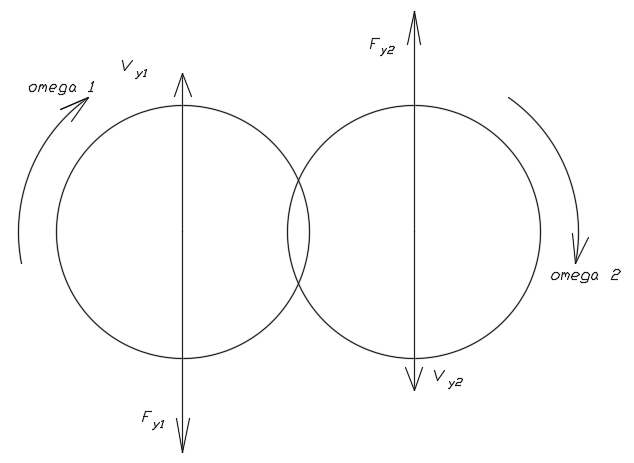
\includegraphics[width=0.5\textwidth]{test_primer} 
	\caption{Пример теста: известны скорости шаров: можем проанализировать направления сил и угловой скорости}
	\label{pic:test_primer}
\end{figure} 


4) Как уже несколько раз было сказано ранее задача очень ресурсоемкая.
Она требует большого количества вычислительной мощности и времени.
Для ускорения программы была написана собственная структура данных, реализующая хэширование.
Проблема заключается в том, что описание работы программы в самом примитивном понимании, когда каждой частице нужно проверить расстояние до кажой другой имеет сложность $O(n^2)$. 
Таким образом, при увеличении числа частиц в 2 раза время расчета программы увеличится в 4 раза. Естественно такой рост невозможен для моделирования большого количества частиц. 
В данной задаче расчет десяти секунд для двухсот сорока шаров доходил до 30-40 часов, чего естественно сложно позволить особенно в промыленной разработке.
Хэширование позволяет уменьшить сложность до $O(n)$. 
Это происходит благодаря тому, что пространство делится на блоки и шар проверяется на пересечении не со всеми другими, присутствующими в расчете, а только с теми что находятся с одним в одном блоке или близлежащих блоках от него.
Таким образом при добавлении новых шаров время работы программы будет $O(n^2)$ только для блоков в которых появился этот шар.
При достаточно большом дроблении общее время для системы будет считаться как $O(n)$. 
Однако, минимальный размер клетки будет ограничен самым большим шаром, учавствующим в расчете, а сетка пересчитываться с определенной переодичностью. 

5) Также удобно сохранять результат работы программы в файл.
Таким образом можно параллельно на разных машинах запустить неограниченное число расчетов и потом проанализировать их одновременно.
А считаться они будут столько же сколько и один расчет, который идет не параллельно.

		\pagebreak
		

\section{Постановка задачи}

\subsection{Механика дробящей среды шаровой мельницы}

Устройство барабанной мельницы довольно подробно представлено в пункте Введение.
Шаровой называется барабанная мельница в которой в качестве дробящего материала используются стальные, чугунные или стеклянные шары.

\begin{figure}[H]
	\centering
	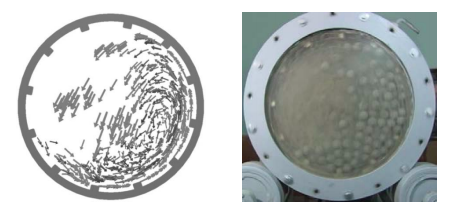
\includegraphics[width=0.7\textwidth]{wall_2mer} 
	\caption{Численное и лабораторное исследование работы шаровой мельницы в двухмерной постановке \cite{mill_foo}.}
	\label{pic:wall_2mer}
\end{figure} 

Постановка задачи для трех степеней свободы является нормальной и широко используется при моделировании режимов работы шаровой мельницы (рисунок \ref{pic:wall_2mer}).

Режим работы шаровой мельницы определяется частотой вращения барабана.
При низкой частоте вращения мельницы шары непрерывно циркулируют, поднимаясь по концентрическим круговым траекториям и скатываясь параллельными слоями каскадом вниз.
Такой режим работы мельницы называется каскадным.

\begin{figure}[H]
	\centering
	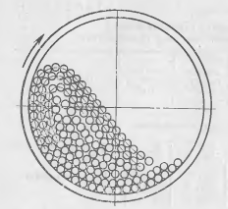
\includegraphics[width=0.5\textwidth]{kaskad_theory} 
	\caption{Схема шаровой нагрузки при каскадном режиме работы мельницы}
	\label{pic:kaskad_theory}
\end{figure} 

По мере повышения частоты вращения мельницы шары по круговым траекториям поднимаются все выше, но режим работы может оставаться каскадным.
Когда, наконец, шары поднимутся до известной, еще большей высоты, определяемой частотой вращения мельницы, они сойдут с круговых траекторий и, как тела, брошенные под углом к горизонту, будут падать по параболическим траекториям водопадом обратно на круговые траектории.
Такой режим работы называется водопадным.

Определение частоты, при которой шар отрывается от стенки мельницы при угле поворота $\alpha$ (рисунок \ref{pic:mill_proec}) происходит аналитически.
В точке А будет справедливо соотношение:
\[
\frac{mv^2}{R} = G \cos (\alpha)
\]
или 
\[
v^2 = Rg \cos (\alpha)
\]
Принимая $v = \dfrac{\pi R n}{30}$, где $n$ -- частота вращения мельницы в минуту, получаем
\begin{equation}
n = \frac{\sqrt{g} \cdot 30}{\pi \cdot \sqrt{R}} \cdot \sqrt{\cos (\alpha)} \text{ об/мин}
\end{equation}

\begin{figure}[H]
	\centering
	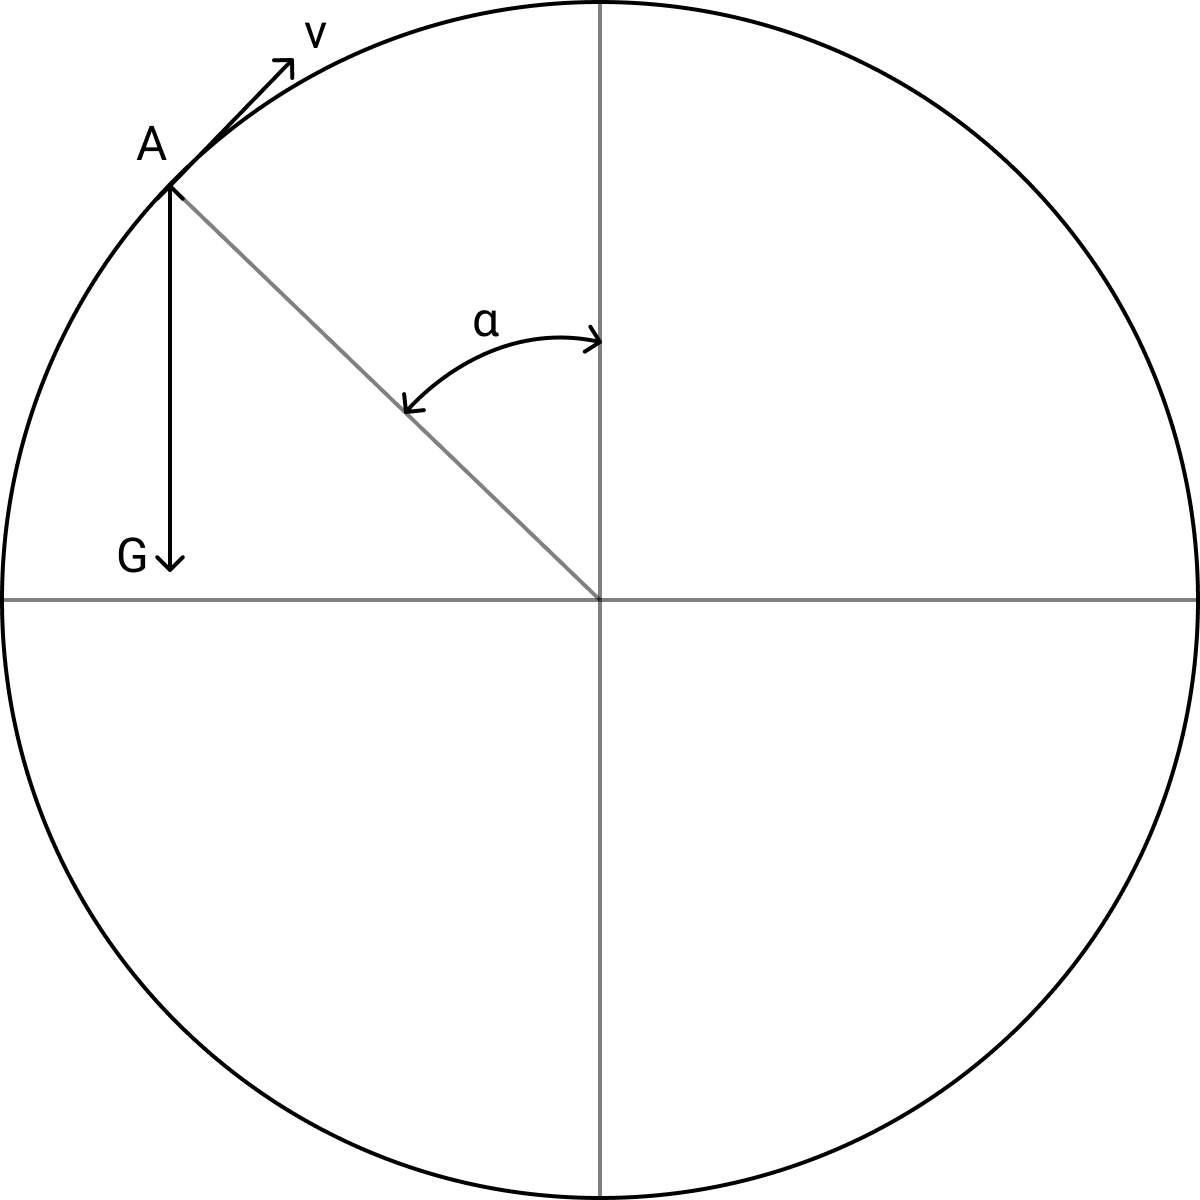
\includegraphics[width=0.5\textwidth]{mill} 
	\caption{Определение частоты вращения мельницы для отрыва чатицы на определенной высоте}
	\label{pic:mill_proec}
\end{figure} 

\begin{figure}[H]
	\centering
	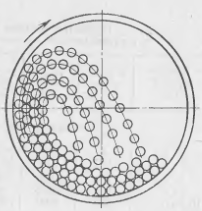
\includegraphics[width=0.5\textwidth]{vodopad_theory} 
	\caption{Схема шаровой нагрузки при водопадном режиме работы мельницы}
	\label{pic:vodopad_theory}
\end{figure} 

Резкого перехода от чисто каскадного режима к чисто водопадному режиму не наблюдается.
Переход происходит постепенно и при промежуточных частотах вращения мельница работает при смешанном каскадно-водопадном режиме.
При таком режиме внешние слои шаров будут падать по параболическим траекториям, но не на свои круговые, а на внутренние слои, скатывающиеся по склону вниз согласно каскадному режиму.
Такой режим считается наиболее предпочтительным, потому что именно при нем наилучшим и наибыстрым образом происходит разрушение частиц руды.

\begin{figure}[H]
	\centering
	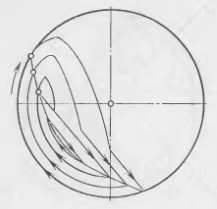
\includegraphics[width=0.5\textwidth]{smeshan_theory} 
	\caption{Схема шаровой нагрузки при смешанном каскадно-водопадном режиме работы мельницы}
	\label{pic:smeshan_theory}
\end{figure} 

Для того чтобы шар поднялся по круговой траектории до наивысшей точки, частота вращения барабана должна вызвать центробежную силу инерции, равную или превосходящую силу тяжести.
При дальнейшем движении после наивысшей точки шар с круговой траектории не сойдет или, как говорят, будет центрифигурировать.

Формула для критической частоты выражается следующим образом

\begin{equation}
\label{freq_kritic}
n_0 = \dfrac{1}{\sqrt[4]{1 - \varphi}} \cdot \dfrac{30 \cdot \sqrt{g}}{\pi \cdot \sqrt{R}}
\end{equation}
где $n_0$ --- частота вращения мельницы, [оборотов в минуту];

$\varphi$ --- отношение объёма, занятого шарами к внутреннему объёму мельницы;

$R$ --- радиус мельницы, [м].

\begin{figure}[H]
	\centering
	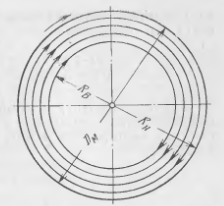
\includegraphics[width=0.5\textwidth]{kritic_theory} 
	\caption{Схема шаровой нагрузки при при превышении критической частоты}
	\label{pic:kritic_theory}
\end{figure} 

\subsection{Реальные параметры}

Для моделирования данной задачи рассматривалась только дробящая среда (без руды). 
В качестве дробящих элементов использовались стальные шары радиусом 20 см.
Коэффициенты трения и скольжения приняты следующим образом
\[
\mu_s = 0.1 \qquad \qquad \qquad \mu_r = 0.05
\]
Коэффициенты диссипации в нормальном и тангенциальном направлениях
\[
\zeta_n = 0.1 \qquad \qquad \qquad \zeta_t = 0.1
\]
Стенка тоже принята стальной и имеет все те же параметры.
Мельница имеет радиус 2.5 м.
В мельницы будет находиться 120 шаров.
Это значит, что по объему она заполнена на 21 \%.

Таким образом можем определить $n_0$ по формуле \ref{freq_kritic}. 
В нашем случае $n_0 = 20$ оборотов в минуту (или 2.1 рад / с).

Шаг по времени равен 10$^{-5}$ секунды.
Каждый эксперимент  проводился в течение 10 секунд.
В реальности расчёт занимал больше времени.


\begin{figure}[H]
	\centering
	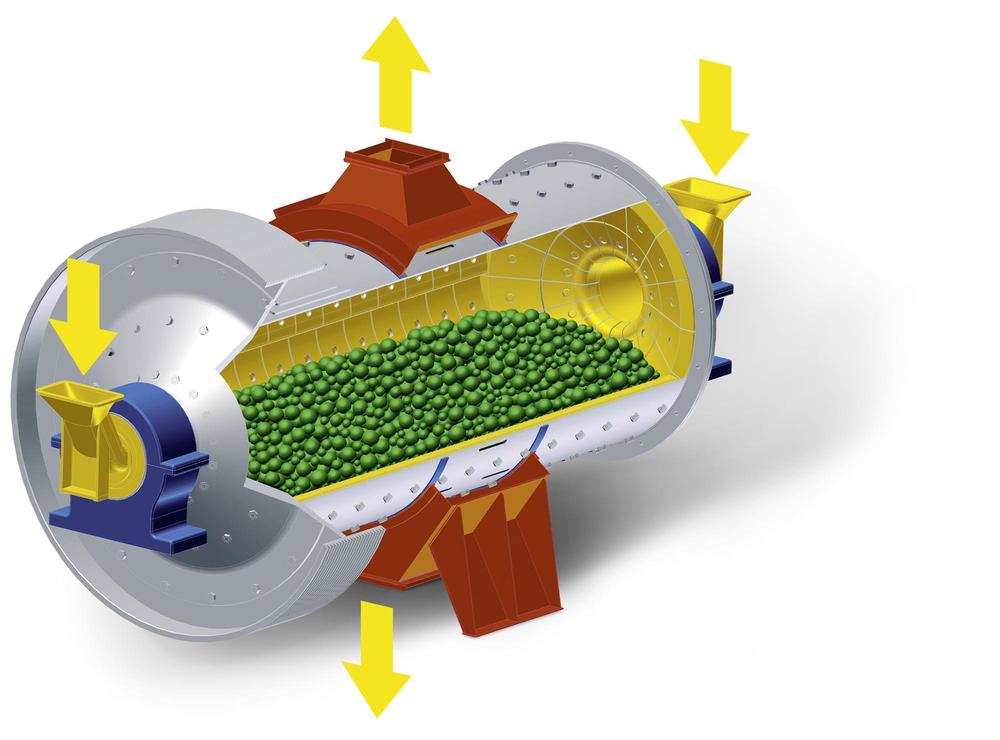
\includegraphics[width=0.5\textwidth]{mill_end} 
	\caption{Схематическое изображеие шаровой мельницы}
	\label{pic:mill_end}
\end{figure} 

\begin{table}[H]
\caption{Реальные значения параметров}
\begin{tabular}{|c|c|}
\hline
Модуль продольной упругости дроби & 2$\times 10^{11}$ Па  \\ 
\hline
Модуль сдвига дроби & 8$\times 10^{10}$ Па \\  
\hline
Плотность дроби & 7800 кг/м$^3$ \\
\hline
Модуль продольной упругости руды & 6$\times 10^{10}$ Па  \\ 
\hline
Модуль сдвига руды & 2.4$\times 10^{10}$ Па \\  
\hline
Плотность руды & 4800 кг/м$^3$ \\
\hline
Минимальная энергия разрушения руды & 0.1 Дж \\
\hline
Параметр прочности & 1 1/Дж \\
\hline
Размеры сита по ширине & 1 м \\
\hline
Размеры сита по ширине & 1 м \\
\hline
Пропускная способность сита & 0.04 м \\
\hline
К-т диссипации в норм-ом направлении & 0.1 \\
\hline
К-т диссипации в танген-ом направлении & 0.1 \\
\hline
К-т трения скольжения & 0.1 \\
\hline
К-т трения качения & 0.05 \\
\hline
Радиус шаровой мельницы & 2.5 м \\
\hline
Изначальный радиус шаров & 0.1 м \\
\hline
Количество шаров & 120 \\
\hline
Процент заполненности мельницы & 21 \% \\
\hline
Шаг по времени & 10$^{-5}$ сек \\
\hline
\end{tabular}
\end{table}

Стоит отметить что часть параметров в этой таблице были найдены эмпирически. 
Например, коэффициенты трения и диссипиации не поддаются точному определению и могут быть получены только при эксперименте при допущении определнных гипотез и для разных наборов материалов и данных могут сильно отличаться.

\subsection{Описание модели рудоразмольной мельницы}

Суммируя описание математической модели и постановки задачи, опишем полноценную модель барабанной мельницы, представленной в данной работе.
В барабанных мельницах материал измельчается внутри полого вращающегося барабана. 
При вращении мелющие тела (шары, стержни) и измельчаемый материал (называемые «загрузкой») сначала движутся по круговой траектории вместе с барабаном, а затем падают по параболе. Часть загрузки, расположенная ближе к оси вращения, скатывается вниз по подстилающим слоям. 
Материал измельчается в результате истирания при относительном перемещении мелющих тел и частиц материала, а также вследствие удара.
Стенка мельницы представлена конечным количеством прямых линий, образующих замкнутый правильный многоугольник.
Внутри стенки находятся элементы стальной дроби и элементы руды.
Элементы дроби выполняют функцию перемалывания частиц руды.
Частицы руды в свою очередь имеют возможность разрушения, основанную на вероятностном подходе и накоплении энергии взаимодействия от соударений в течении жизненного цикла частицы (пункт \ref{sub:break_model}).
Так же промоделирована подача новой руды в расчитываемую модель, которая происходит с некоторой периодичностью подобранной эмпирическим путем.
В центре мельницы также организовано сита.
При попадании особо малых частиц в область сита частицы выпадают из расчета (условие \ref{eq:exit}).
Скорость вращения мельницы варьируется.
Стенка имеет те же механические параметры, что и стальная дробь.

Мельнице, как уже сказано выше, подается материал руды через одну цапфу.
Материал подается с периодичностью заданной изначально и найденной эмпирически для конкретной модели.
Область в которую подается материал считается наименее загруженной (если мельница вращается по часовой стрелке, значит такой областью будет правый верхний угол).
Размер появляющейся частицы считается жестко заданным и фиксированным
В данной задаче рассматривается двухмерная постановка поэтому можно считать, что рассматривается вращение шаров находящихся на удалении от обоих цапф (по середине как показано на рисунке \ref{pic:mill_end}).
Когда частица достигает определенного размера $r_{s}$ или меньшего, то при попадании в область сита (будем считать что оно находится в центре мельницы около оси, вокруг которой происходит вращение):
\begin{align}
\label{eq:exit}
r &< r_s \\
x_{s-l} &< x_b < x_{s-r} \\
y_{s-d} &< y_b < y_{s-u}
\end{align}
частица будет исчезать из расчета. Принимается, что сито прямоугольное.

$x_{s-l}$ -- координата левой границы сито по оси OX;

$x_{s-r}$ -- координата правой границы сито по оси OX;

$x_b$ -- координата центра шара по оси OХ;

$y_{s-d}$ -- координата нижней границы сито по оси OY;

$y_{s-u}$ -- координата верхней границы сито по оси OY;

$y_b$ -- координата центра шара по оси OY.




\pagebreak

\section{Результаты моделирования}

\subsection{Каскадный режим работы}

При частоте вращения мельницы 0.2 рад / с (1.9 оборотов в минуту) можем наблюдать каскадный режим работы.
Графики изменения энергии (этот и следующие: \ref{pic:kaskad_energy}, \ref{pic:vodopad_energy}, \ref{pic:smeshan_energy}, \ref{pic:kritic_energy}) показывает, что диссипирующая система, которая получает постоянную подпитку энергией извне (стенка крутится, тем самым разгоняя шары) приходит к примерно равновесному по энергии состоянию.

\begin{figure}[H]
	\centering
	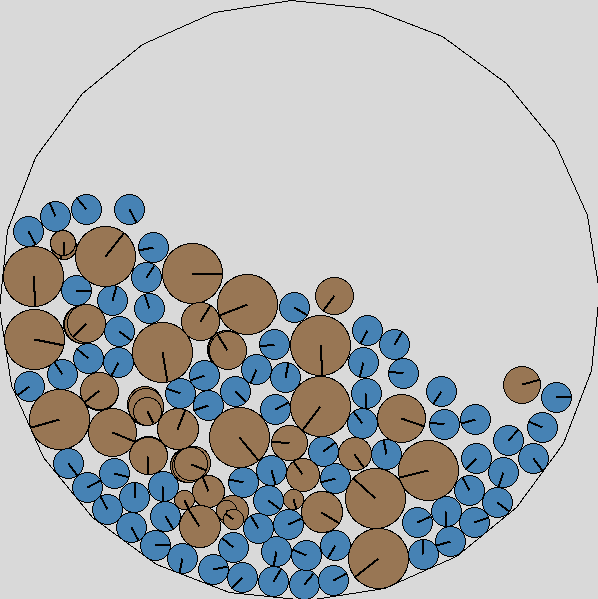
\includegraphics[width=0.5\textwidth]{kaskad_result} 
	\caption{Экспериментальная схема шаровой нагрузки при каскадном режиме работы мельницы}
	\label{pic:kaskad_result}
\end{figure} 

\begin{figure}[H]
	\centering
	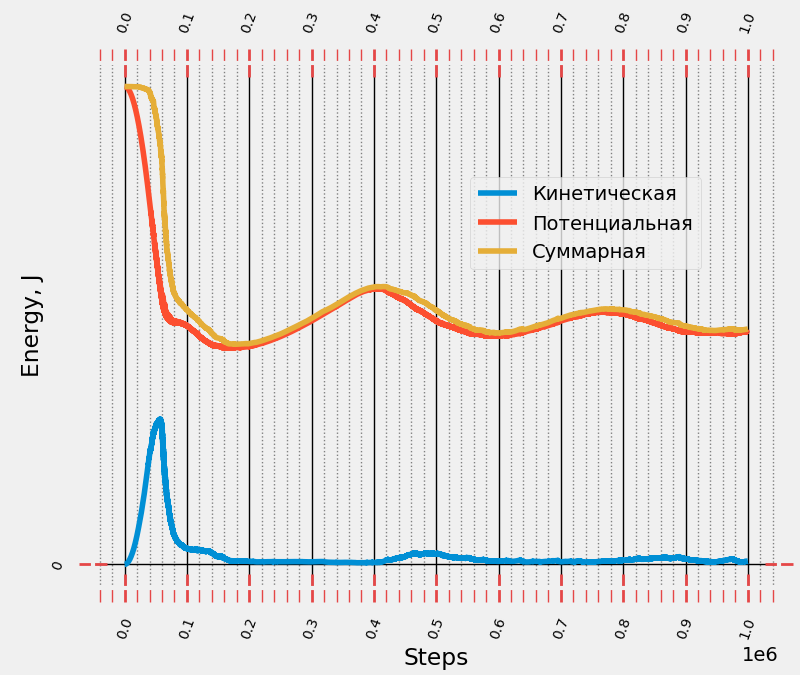
\includegraphics[width=0.5\textwidth]{kaskad_energy}
	\caption{График изменения энергии во времени при каскадном режиме работы мельницы}
	\label{pic:kaskad_energy}
\end{figure} 

\subsection{Водопадный режим работы}

Данный режим работы достигается при 1.8 рад / с (17.19 оборотов в минуту).
Для более выразительной картины данного режима (рисунок \ref{pic:vodopad_theory}) количество шаров увеличено до 240. 
Таким образом заполненность мельницы увеличивается до 42 процентов что близко к максимальному кпд. 

\begin{figure}[H]
	\centering
	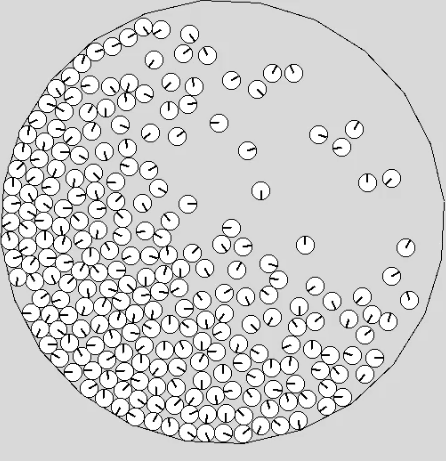
\includegraphics[width=0.5\textwidth]{vodopad_result} 
	\caption{Экспериментальная схема шаровой нагрузки при водопадном режиме работы мельницы}
	\label{pic:vodopad_result}
\end{figure} 

\begin{figure}[H]
	\centering
	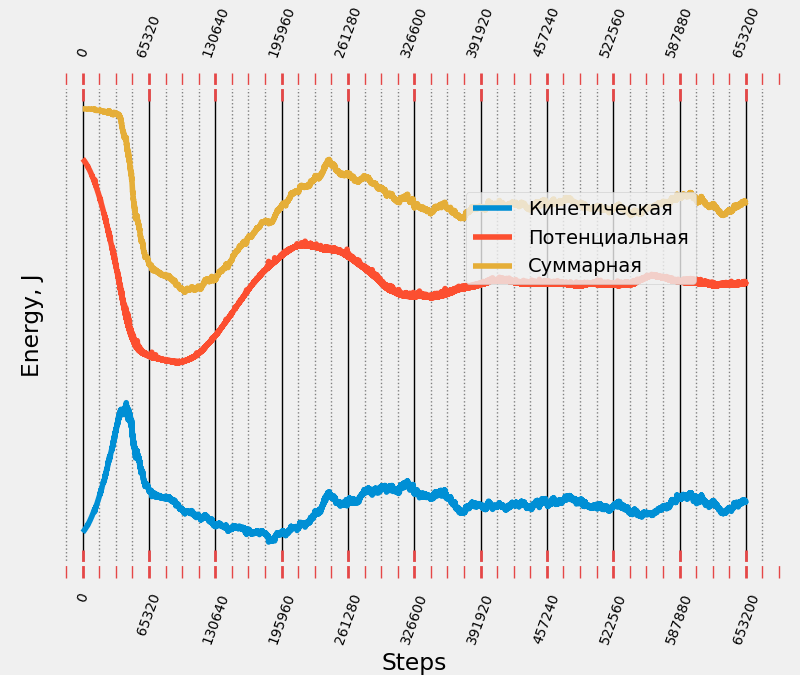
\includegraphics[width=0.5\textwidth]{vodopad_energy} 
	\caption{График изменения энергии во времени при водопадном режиме работы мельницы}
	\label{pic:vodopad_energy}
\end{figure} 

\subsection{Смешанный каскадно-водопадный режим работы}

Данный режим работы достигается при 1.5 рад / с (14.32 оборотов в минуту).
Как уже было сказано ранее этот режим является наиболее удачным для измельчения руды.
И это видно: часть шаров перекатывается, а часть шаров падает на них сверху.
Это и создает ударную нагрузку, необходимую для разрушения.

\begin{figure}[H]
	\centering
	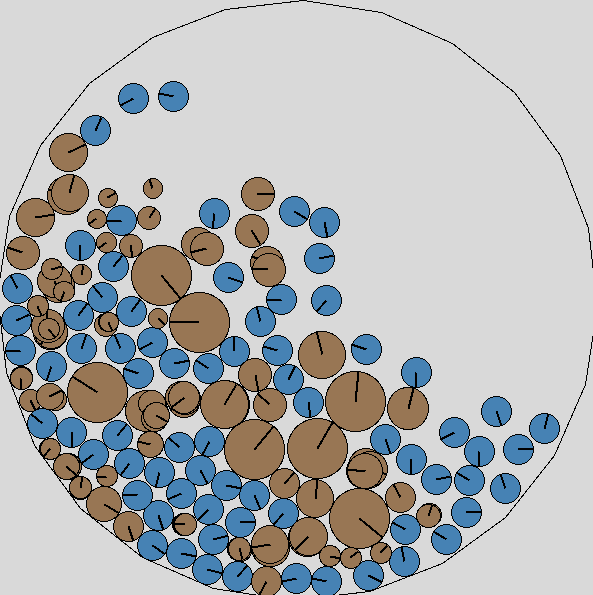
\includegraphics[width=0.5\textwidth]{smeshan_result} 
	\caption{Экспериментальная схема шаровой нагрузки при смешанном каскадно-водопадном режиме работы мельницы}
	\label{pic:smeshan_result}
\end{figure} 

\begin{figure}[H]
	\centering
	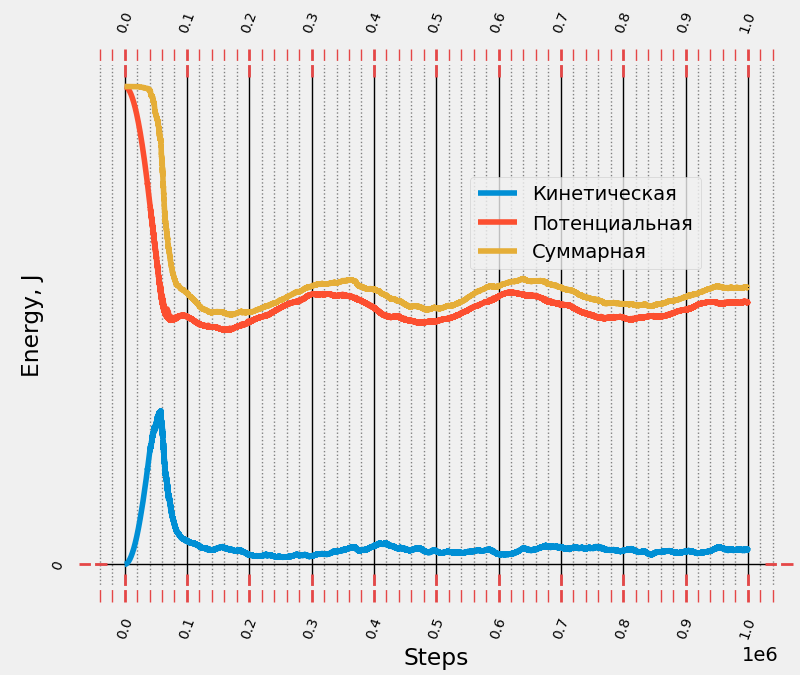
\includegraphics[width=0.5\textwidth]{smeshan_energy} 
	\caption{График изменения энергии во времени при смешанном каскадно-водопадном режиме работы мельницы}
	\label{pic:smeshan_energy}
\end{figure} 

\subsection{Режим работы мельницы при закритической частоте}

Для более быстрого установления характерной картины (рисунок \ref{pic:kritic_theory}) выберем частоту работы мельницы, превышаюшую теоретическую в несколько раз.
В данном примере мельница врашается со скоростью 10 рад / с (95.49 оборотов в минуту).

\begin{figure}[H]
	\centering
	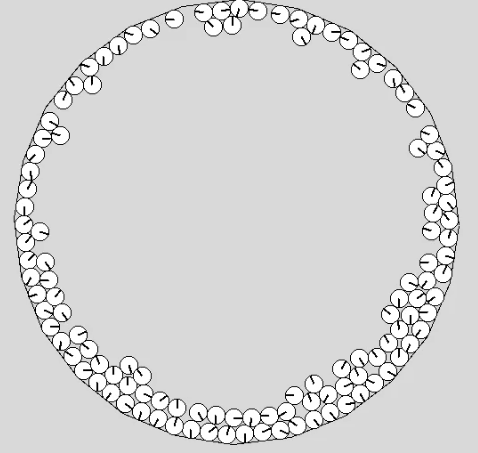
\includegraphics[width=0.5\textwidth]{kritic_result} 
	\caption{Экспериментальная схема шаровой нагрузки при при превышении критической частоты}
	\label{pic:kritic_result}
\end{figure} 

\begin{figure}[H]
	\centering
	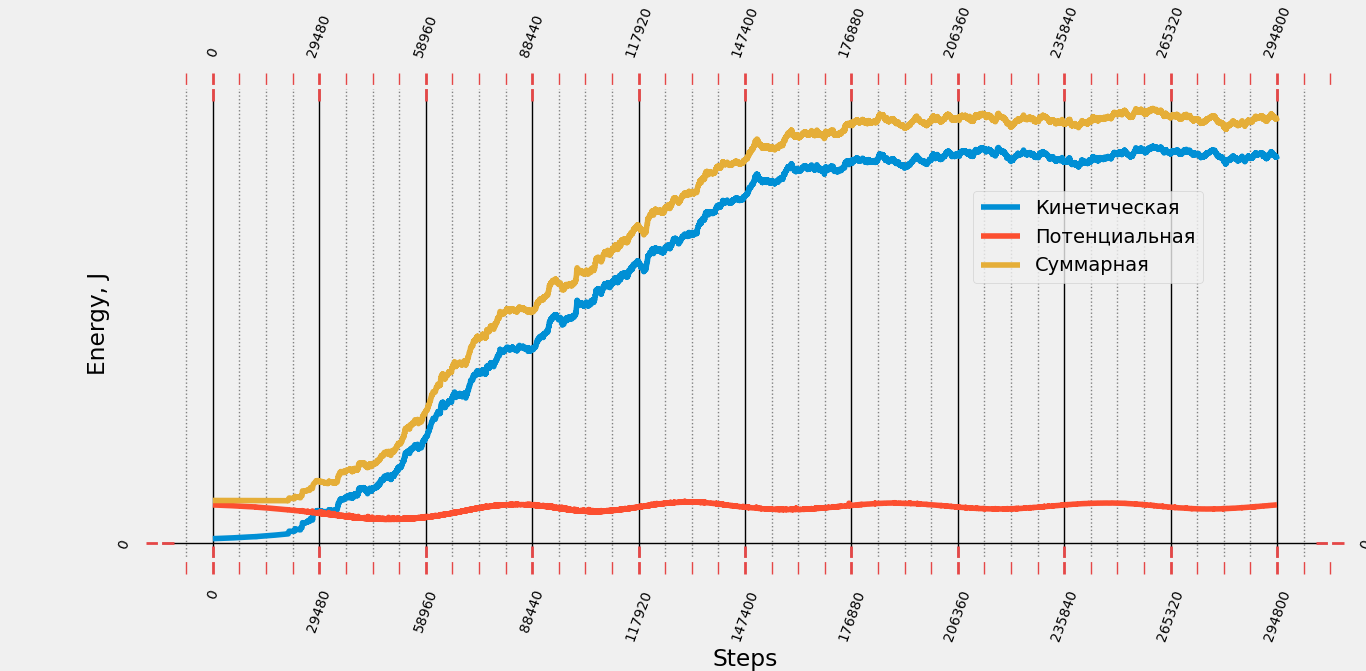
\includegraphics[width=0.5\textwidth]{kritic_energy} 
	\caption{График изменения энергии во времени при при превышении критической частоты}
	\label{pic:kritic_energy}
\end{figure} 


		\pagebreak
		
	\section*{ЗАКЛЮЧЕНИЕ}
		\addcontentsline{toc}{section}{ЗАКЛЮЧЕНИЕ}

В представленной работе изучен метод дискретных элементов, а также была разработана математическая модель динамики частиц дроби в шаровой рудоразмольной мельнице.
В качестве примера применимости и работоспособности данной математической модели планируется провести серию численных экспериментов по моделированию разрушения руды в барабане мельницы для набора режимов ее работы.
Разработанная модель позволяет исследовать режимы работы рудоразмольной мельницы.
Такой подход позволит сэкономить много денежных и ресурсных запасов, отказавшись от проведения достаточно дорогих и сложных экспериментов.

		\pagebreak

		
\begin{thebibliography}{99}
\addcontentsline{toc}{section}{СПИСОК ИСПОЛЬЗОВАННЫХ ИСТОЧНИКОВ}
\bibitem{cundall} Cundall P. A., Strack O. D. L. A discrete numerical model for granular assemblies //geotechnique. – 1979. – Т. 29. – №. 1. – С. 47-65.
\bibitem{mde_smth} Арсентьев В. А. и др. Методы динамики частиц и дискретных элементов как инструмент исследования и оптимизации процессов переработки природных и техногенных материалов //Обогащение руд. – 2010. – №. 1. – С. 30-35.
\bibitem{hard_aglomerath} Chen J. Discrete element method for 3D simulations of mechanical systems of non-spherical granular materials //The University of Electro. – 2012.
\bibitem{some} Ревуженко А. Ф., Клишин С. В., Бегляков В. Ю. Использование метода дискретных элементов при исследовании дилатансионных характеристик сыпучей среды //Актуальные проблемы современного машиностроения: сборник трудов Международной научно-практической конференции, г. Юрга, 11-12 декабря 2014 г.—Томск, 2014. – 2014. – С. 90-93.
\bibitem{aglomerath} Караваев А. С., Копысов С. П., Сармакеева А. С. Моделирование динамики произвольных тел методом дискретных элементов //Вестник Удмуртского университета. Математика. Механика. Компьютерные науки. – 2015. – Т. 25. – №. 4. – С. 473-482.
\bibitem{another_hard} Quist J. DEM modelling and simulation of cone crushers and high pressure grinding rolls. – Chalmers University of Technology, 2017.
\bibitem{priklad} Верзилина О. А. Применение метода дискретных элементов для моделирования виброударных систем //Экономика. Информатика. – 2018. – Т. 45. – №. 1.
\bibitem{china_mill} Xu J. et al. Quasi-real-time simulation of rotating drum using discrete element method with parallel GPU computing //Particuology. – 2011. – Т. 9. – №. 4. – С. 446-450.
\bibitem{mill_book} Андреев С. Е., Перов В. А., Зверевич В. В. Дробление, измельчение и грохочение полезных ископаемых. – Недра, 1980. – С. 415.
\bibitem{mill_smth} Чижик Е. Ф., Соколов В. И. Концепция измельчения руд в шаровых барабанных мельницах //Горный информационно-аналитический бюллетень (научно-технический журнал). – 2005. – №. 4.
\bibitem{friction_calibration} Syed Z., Tekeste M., White D. A coupled sliding and rolling friction model for DEM calibration //Journal of Terramechanics. – 2017. – Т. 72. – С. 9-20.
\bibitem{pruzhina} Полищук И. В., Бобков С. П. Использование метода дискретных элементов для моделирования процесса неупругого деформирования //Вестник Ивановского государственного энергетического университета. – 2014. – №. 6. – С. 71-74.
\bibitem{many_pruzhina} Бобков С. П., Полищук И. В. Исследование процесса упругого деформирования с использованием метода дискретных элементов //Вестник Ивановского государственного энергетического университета. – 2014. – №. 5. – С. 47-50.
\bibitem{razr} Белоглазов И. И., Иконников Д. А. Применение метода дискретных элементов для моделирования процесса измельчения горных пород в щековой дробилке //Известия высших учебных заведений. Приборостроение. – 2016. – Т. 59. – №. 9.
\bibitem{mill_foo} Сысоев Н. И., Маляров П. В., Скляров Е. В. Совершенствование резинометаллической футеровки барабанной мельницы на основе учета характера движения шаровой загрузки //Известия высших учебных заведений. Северо-Кавказский регион. Технические науки. – 2012. – №. 3.

\end{thebibliography}
		\pagebreak
\end{document}